\documentclass[10pt, a4paper, italian]{article}
\usepackage[T1]{fontenc}
\usepackage[utf8]{inputenc}
\usepackage{amsmath, amssymb, amsthm, thmtools, amsfonts, mathtools}
\usepackage{nicefrac}
\usepackage{calc}
\usepackage[pdftex, hyperindex, plainpages=false]{hyperref}
\usepackage[nameinlink]{cleveref} %load before classicthesis (clash)
%\usepackage[nochapters,pdfspacing]{classicthesis}
\usepackage{siunitx}
\usepackage[siunitx]{circuitikz}

\usepackage[a4paper]{geometry}
\usepackage{float}
\usepackage{mdframed}
\usepackage{titling}
\usepackage{booktabs}
\usepackage{graphicx}
\usepackage{caption, subcaption}
\usepackage{xcolor}
\usepackage[italian]{babel}
\usepackage{pgfplots}
\usepackage{listings}
%\usepackage{lmodern}
\usepackage{url}
\usepackage{enumitem}
\usepackage{tikz} %loads after classicthesis (xcolor incompat)

% lets graphicx know path where figures to be included are found
\graphicspath{{../figs/}}
\makeatletter
\def\input@path{{../figs/}}
%or: \def\input@path{{/path/to/folder/}{/path/to/other/folder/}}
\makeatother

% tikz pgf plots setup
\usepgfplotslibrary{external}
\pgfplotsset{compat=1.15}
%\tikzexternalize

% spaces and significant digits/figures for measurements
\sisetup{free-standing-units, space-before-unit, number-unit-product = \;,
scientific-notation = false, round-mode = figures, round-precision = 1,}

% turns all (hyperlinked) references black [default is blue]
\hypersetup{
	linktoc=all,
	colorlinks=true,
	linkcolor=black
}

% code listings config
%\lstset{
%language=Python,
%basicstyle=\ttfamily,
%columns=fullflexible,
%keepspaces=true,
%}

% mdframed (for boxed text) configuration
\mdfsetup{linewidth=0.6pt}

% Default fixed font does not support bold face
\DeclareFixedFont{\ttb}{T1}{txtt}{bx}{n}{12} % for bold
\DeclareFixedFont{\ttm}{T1}{txtt}{m}{n}{12}  % for normal

% Custom colors
\usepackage{color}
\definecolor{deepblue}{rgb}{0,0,0.5}
\definecolor{deepred}{rgb}{0.6,0,0}
\definecolor{deepgreen}{rgb}{0,0.5,0}

% Commands 
\newcommand{\executeiffilenewer}[3]{%
	\ifnum\pdfstrcmp{\pdffilemoddate{#1}}%
		{\pdffilemoddate{#2}}>0%
	{\immediate\write18{#3}}\fi%
}
% input .svg --> .pdf_tex graphs
%\newcommand{\includesvg}[1]{%
%	\executeiffilenewer{#1.svg}{#1.pdf}%
%	{inkscape -z -D --file=#1.svg %
%	--export-pdf=#1.pdf --export-latex}%
%	\input{#1.pdf_tex}%
%}
% Thanks UniPi's Department of Physics E. Fermi
\newcommand{\thanksdf}{(\thanks{Dipartimento di Fisica E.~Fermi,%
Universit\`a di Pisa - Pisa, Italy.}\;)}

% hyperlink to email address
\newcommand{\mail}[1]{\href{mailto:#1}{\textsf{#1}}}

% \vec for bold vectors, instead of overarrows (now "\arrvec")
\let\arrvec=\vec
\renewcommand{\vec}[1]{\boldsymbol #1}
% replaces straight phi with slanted phi
\renewcommand{\phi}{\varphi}
% replaces straight eps with curved epsilon
\newcommand{\eps}{\varepsilon}
% abbreviation for (sub_/super^)scripts of \lim, \sum,... in inline math
\newcommand{\ds}{\displaystyle}

% blackboard/number set letters
\newcommand{\CC}{\mathbb C}
\newcommand{\HH}{\mathbb H}
\newcommand{\KK}{\mathbb K}
\newcommand{\NN}{\mathbb N}
\newcommand{\PP}{\mathbb P}
\newcommand{\QQ}{\mathbb Q}
\newcommand{\RR}{\mathbb R}
\newcommand{\ZZ}{\mathbb Z}

\newcommand{\Abs}[1]{{\left\Vert #1\right\Vert}}
\newcommand{\enclose}[1]{{\left( #1 \right)}}
\newcommand{\Enclose}[1]{{\left[ #1 \right]}}
\newcommand{\floor}[1]{\left\lfloor #1 \right\rfloor}
\newcommand{\ceil}[1]{\left\lceil #1 \right\rceil}
\newcommand{\To}{\rightrightarrows}

% Math operators
\DeclareMathOperator{\divergence}{div}
\renewcommand{\div}{\divergence}
\DeclareMathOperator{\Imaginarypart}{Im}
\renewcommand{\Im}{\Imaginarypart}
\DeclareMathOperator{\Realpart}{Re}
\renewcommand{\Re}{\Realpart}
%\DeclareMathOperator{\arg}{arg}
\DeclareMathOperator{\tg}{tg}
\DeclareMathOperator{\arctg}{arctg}
\DeclareMathOperator{\settsinh}{settsinh}
\DeclareMathOperator{\settcosh}{settcosh}
\DeclareMathOperator{\tr}{tr}
\DeclareMathOperator{\im}{im}
\DeclareMathOperator{\sgn}{sgn}
\DeclareMathOperator{\diag}{diag}

\DeclarePairedDelimiter{\norm}{\lVert}{\rVert}
\DeclarePairedDelimiter{\scalar}{\langle}{\rangle}

% Logarithm with arbitrary base.
% -> log_10
\newcommand{\llog}[1][10]{\log_{#1}}

% Absolute value.
% -> |x|
\newcommand{\abs}[1]{\left| #1 \right|}

% Powers.
% -> x^a
\newcommand{\power}[2][2]{\left( #2 \right)^{#1}}

% Square.
% -> x^2
\newcommand{\sq}[1]{\power[2]{#1}}

% Expansion of the binomial coefficient.
% -> n1!/(n2!(n1 - n2)!)
\newcommand{\binomexpr}[2]{\frac{#1!}{#2!(#1 - #2)!}}

% Expression evaluation at a given point with square brackets.
% -> [x]_{a}
\newcommand{\at}[2]{\left[ #1\right]_{\makebox[-1pt][l]{${\scriptstyle#2}$}}}

% Expression evaluation in an interval.
% -> [x] _{a}^{b}
\newcommand{\eval}[3]{\left.#1%
  \right|_{\makebox[-1pt][l]{${\scriptstyle#2}$}}^{\makebox[-1pt][l]{${\scriptstyle#3}$}}}

% Upright d in math mode (for differentials).
% -> d
\newcommand{\ud}{\mathrm{d}}

% Differential.
% -> dx
\newcommand{\diff}[1][x]{\,\ud{#1}}

% Base command for defining derivatives.
% -> df/dx or d^kf/dx^k
\newcommand{\basederivative}[4][]{%
  \displaystyle%
  \ifx\\#1\\\frac{#4#2}{#4#3}%
  \else%
  \frac{#4^#1#2}{#4#3^#1}%
  \fi%
}

% Total derivative.
% -> df/dx(x) or d^kf/dx^k(x)
\newcommand{\td}[4][]{%
  \basederivative[#1]{#2}{#3}{\ud}%
  \ifx\\#4\\%
  \else%
  \mkern-4mu\left(#4\right)%
  \fi%
}

% Partial derivative.
% -> df/dx(x) or d^kf/dx^k(x)
\newcommand{\pd}[4][]{%
  \basederivative[#1]{#2}{#3}{\partial}%
  \ifx\\#4\\%
  \else%
  \mkern-4mu\left(#4\right)%
  \fi%
}

\newcommand{\intinf}{\int_{-\infty}^{\infty}\!\!\!}

\newcommand{\cinterval}[2]{\left[\, #1,~#2 \,\right]}

\newcommand{\linterval}[2]{\left[\, #1,~#2 \,\right)}

\newcommand{\rinterval}[2]{\left(\, #1,~#2 \,\right]}

\newcommand{\ointerval}[2]{\left(\, #1,~#2 \,\right)}

\newcommand{\prob}[1]{\displaystyle P\left(#1\right)}

\newcommand{\pvalue}{\emph{$p$-value}}

\newcommand{\cond}{\,|\,}

\newcommand{\expect}[1]{\displaystyle E\left[#1\right]}

\newcommand{\mom}[2][]{\displaystyle {\cal M}_{#2}\ifx\\#1\\\else(#1)\fi}

\newcommand{\momalg}[1]{\displaystyle \lambda_{#1}}

\newcommand{\momcen}[1]{\displaystyle \mu_{#1}}

\newcommand{\skewness}{\displaystyle \gamma_1}

\newcommand{\kurtosis}{\displaystyle \gamma_2}

\newcommand{\charf}[1][x]{\phi_{#1}}

\newcommand{\momgenf}[1][x]{M_{#1}}

\newcommand{\fwhm}{{\scriptstyle \textsc{FWHM}}}

\newcommand{\hwhm}{{\scriptstyle \textsc{HWHM}}}

\newcommand{\median}{\mu_{\nicefrac{1}{2}}}

\newcommand{\var}[1]{\ensuremath{\text{Var}\left(#1\right)}}

\newcommand{\cov}[2]{\ensuremath{\text{Cov}\left(#1, #2\right)}}

\newcommand{\corr}[2]{\ensuremath{\text{Corr}\left(#1, #2\right)}}

\newcommand{\like}{\mathcal L}

\newcommand{\likelihood}[2][]{\like\ifx\\#2\\\else(#2\ifx\\#1\\\else;#1\fi)\fi}

\newcommand{\chisq}{\ensuremath{\chi^2}}

\newcommand{\chisquare}[2][]{\chisq\ifx\\#2\\\else(#2\ifx\\#1\\\else;#1\fi)\fi}

\newcommand{\loglikelihood}[2][]{\log\likelihood[#1]{#2}}

\newcommand{\pdf}[3][]{#2(#3\ifx\\#1\\\else;#1\fi)}

\newcommand{\binomialpdf}[2][]{\pdf[#1]{\mathcal B}{#2}}

\newcommand{\multinomialpdf}[2][]{\pdf[#1]{\mathcal M}{#2}}

\newcommand{\poissonpdf}[2][]{\pdf[#1]{\mathcal P}{#2}}

\newcommand{\uniformpdf}[2][]{\pdf[#1]{u}{#2}}

\newcommand{\exponentialpdf}[2][]{\pdf[#1]{\varepsilon}{#2}}

\newcommand{\gausspdf}[2][]{\pdf[#1]{N}{#2}}

\newcommand{\chisquarepdf}[2][]{\pdf[#1]{\wp}{#2}}

\newcommand{\cauchypdf}[2][]{\pdf[#1]{c}{#2}}

\newcommand{\erf}[1]{\ensuremath{\text{erf}\left(#1\right)}}

\newcommand{\dccases}[4][]{#2 \ifx\\#2\\\else=\fi %
  \begin{cases}
    \displaystyle #3 & \text{per variabili discrete}\\
    \displaystyle #4 & \text{per variabili continue}#1
  \end{cases}
}
% sub/super-scriptable for all symbol as math operator 
\newcommand\Scaleforall[1]{\vcenter{\hbox{\scalefont{#1}$\forall$}}}

\DeclareMathOperator*\forevery{%
  \vphantom\sum
  \mathchoice{\Scaleforall{2}}{\Scaleforall{1.4}}{\Scaleforall{1}}{\Scaleforall{0.75}}}
\geometry{left=2cm, right=2cm, top=2cm, bottom=2cm}

% indexes subsections with letters, sections with numbers (1.a, 1.b, ...)
\renewcommand{\thesubsection}{\thesection.\alph{subsection}}

% lets graphicx know path where figures to be included are found
\graphicspath{{../figs/}}

\author{Gruppo 1.AC \\ Bernardo Tomelleri}
\title{Es06A: Oscillatore sinusoidale a ponte di Wien con OpAmp}
\begin{document}
\date{9 gennaio 2022}
\maketitle

\tableofcontents
\section{Misura componenti dei circuiti}
\begin{table}[htbp]
\centering
\begin{tabular}{cccccc}
\toprule
Resistenze $[\si{k\ohm}]$ & $R$ & $\sigma R$ & Capacità $[\si{n\F}]$ & $C$ &
$\sigma C$ \\
\midrule
\midrule
$R_1$	  & 9.95	& 0.08	 & $C_1$ & 10.4		 & 0.4 \\
$R_2$	  & 9.92	& 0.08 	 & $C_2$ & 10.5		 & 0.4 \\
$R_3$	  & 9.93	& 0.08	 & & & \\
$R_4$	  & 9.93	& 0.08	 & & & \\
$R_5$	  & 9.95	& 0.08	 & & & \\
$R$		  & 9.53	& 0.08	 & & & \\
\bottomrule     
\end{tabular}
\caption{Valori di resistenza e capacità misurate per i componenti dei
circuiti studiati. \label{tab: rcmes}}
\end{table}

Riportiamo per completezza anche i valori delle tensioni di alimentazione
continue per l'op-amp misurate con il multimetro
\begin{align*}
V_{CC} &= 4.99 \pm 0.03 \si{\V} \\
V_{EE} &= -4.99 \pm 0.03 \si{\V}
\end{align*}

Per tutto il resto della trattazione come ampiezze dei segnali si intendono
misurate non ``picco - picco'', a meno che non venga esplicitato altrimenti.

\subsection{Nota sul metodo di fit}
Per determinare i parametri ottimali e le rispettive covarianze si \`e
implementato in \verb+Python+ un algoritmo di fit basato sui minimi quadrati
mediante la funzione \emph{curve\_fit} della libreria \texttt{SciPy}.

%=======================
\section{Apparato di misura del guadagno ad anello chiuso}
Si è montato il circuito per la misura del loop-gain
$\bar{L}(j\omega) = \beta(j\omega) \bar{A}$ nel nostro generatore di
onde sinusoidali come quello proposto nello schema in \cref{fig: aloopschm}

\begin{figure}[htbp]
    \centering
	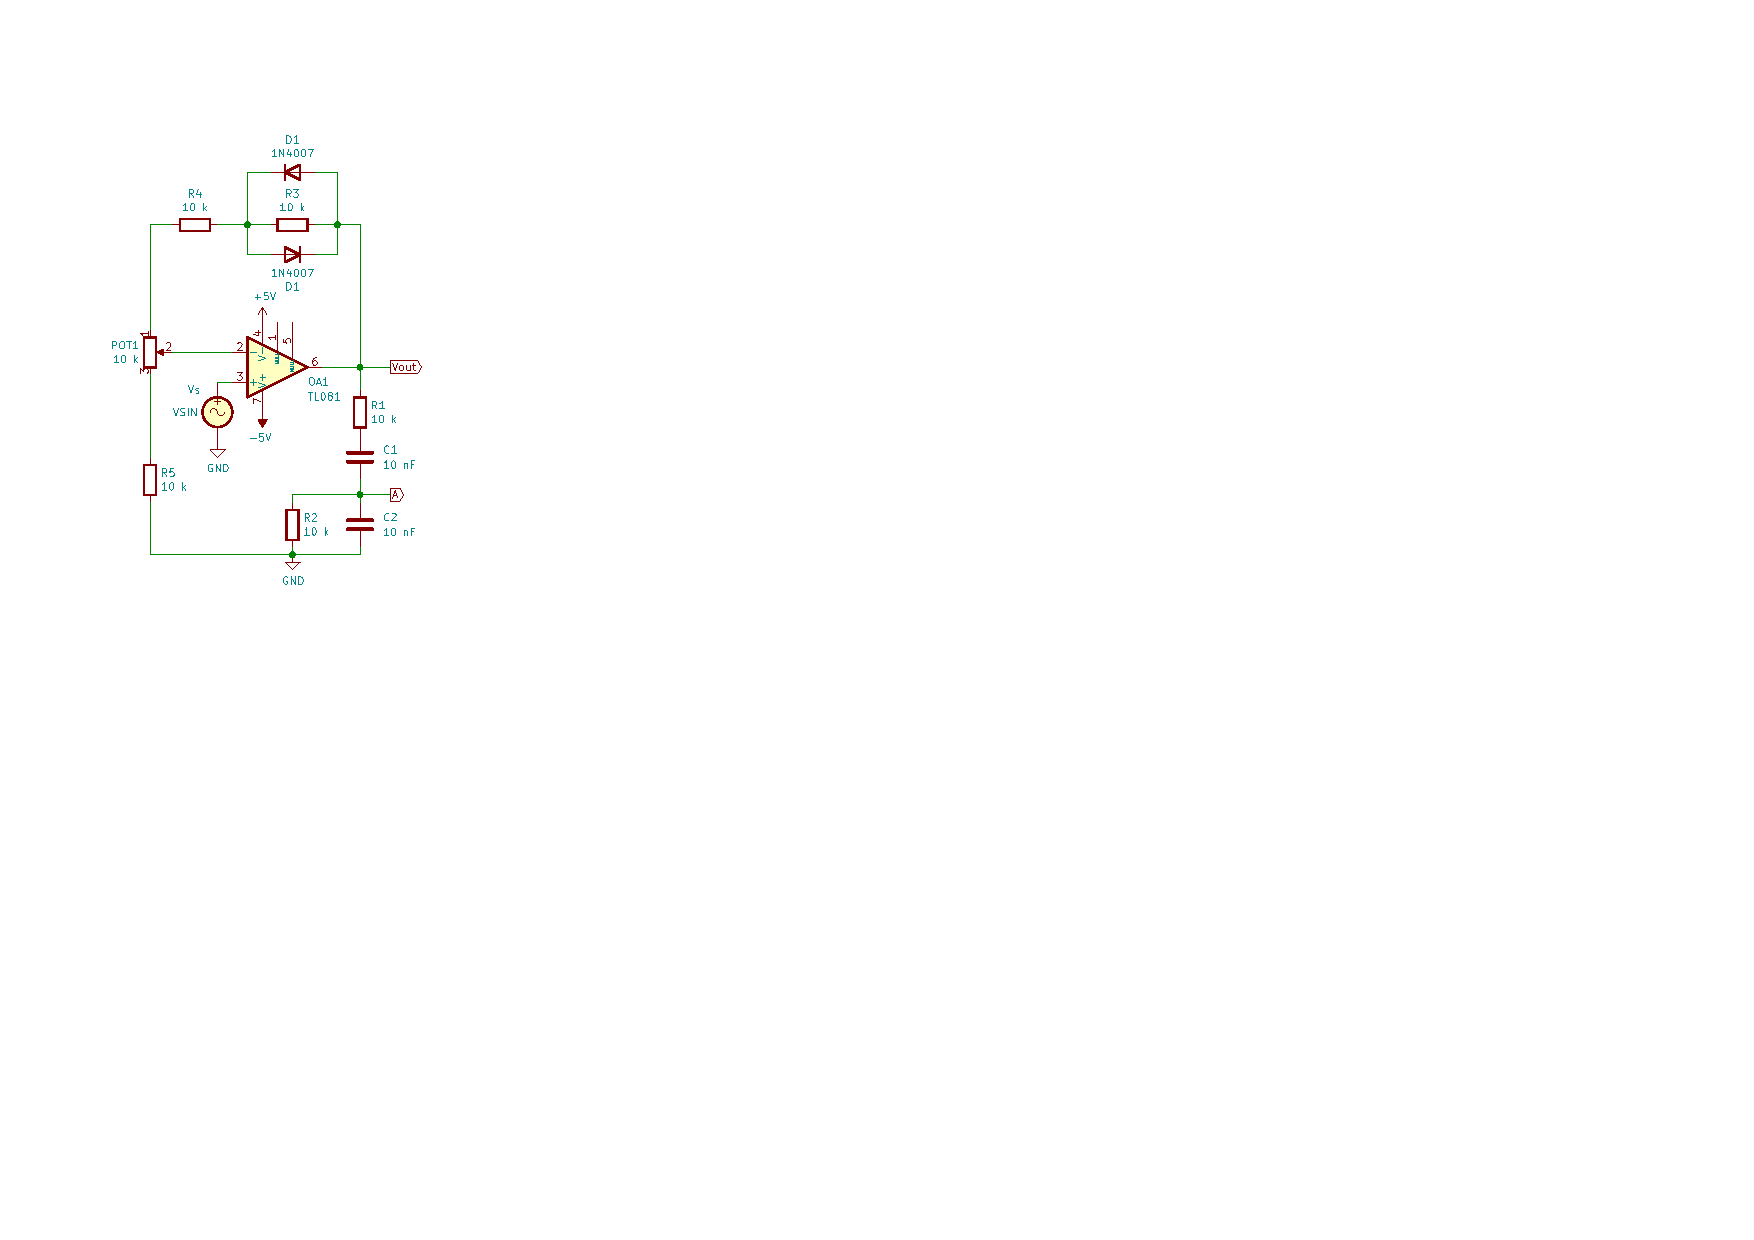
\includegraphics[scale=1.2]{aloopschm}
    \caption{Schema circuitale dell'amplificatore di carica costruito.
    \label{fig: aloopschm}}
\end{figure}

Il circuito è formato da un amplificatore non-invertente con guadagno
indipendente dalla frequenza (trascurando la presenza e risposta non lineare
dei diodi in parallelo a $R_3$ - che consideriamo dei circuiti aperti - dal
momento che supponiamo di lavorare con $V\ped{out} \sim V_{R_3}$ vincolato ad
essere in modulo minore rispetto alla tensione caratteristica del regime di
conduzione in cui questi svolgono un ruolo $V_\gamma \sim \SI{0.7}{\V}$)
\begin{equation}\label{eq: A}
A  = 1 + \frac{(1 - p)R + R_3 + R_4}{pR + R_5}
\end{equation}
in cui il parametro $p \in [0,1]$ è stato introdotto per indicare la posizione
del contatto strisciante in POT1, o meglio la frazione di resistenza
totale $R$ del potenziometro ideale che si trova tra il terminale centrale e
la resistenza $R_5$ (dunque massa). Quindi, per costruzione, quando $p = 0$
il trimmer del potenziometro è girato tutto verso il basso ($R_5$), mentre per
$p = 1$ è rivolto verso l'alto ($R_4$).

A questo si aggiunge un anello di feedback ``positivo'' il cui guadagno è dato
dal rapporto di partizione
\begin{equation} \label{eq:loop-gain-beta}
\beta(s) = \frac{Z_P}{Z_S + Z_P} = \frac{1}{Z_S/Z_P + 1}
\end{equation}
tra un'impedenza RC ``serie'' $Z_S$ e un'impedenza ``parallelo'' $Z_P$,
ovverosia
\begin{align*}
Z_S &= R_1 + \frac{1}{s C_1} = R_1 \frac{s + \omega_1}{s} \\
Z_P &= \frac{R_2}{1 + s R_2 C_2} = R_2 \frac{\omega_2}{s + \omega_2}
\end{align*}
dove abbiamo indicato $\omega_1 = 1/(R_1 C_1)$ e con $\omega_2 = 1/(R_2 C_2)$.
Espandendo in termini delle singole resistenze e pulsazioni possiamo riscrivere
il fattore di feedback
\begin{equation}
\beta(s) = \frac{1}{1 + Z_S/Z_P} =
\frac{1}{1 + \frac{R_1}{R_2} \frac{(s + \omega_1)(s + \omega_2)}{s \omega_2}} =
\frac{R_2}{R_1} \frac{s \omega_2}{\omega_1 \omega_2 + s^2 +
\left[\omega_{1} + \omega_{2} \left(1 + \frac{R_2}{R_{1}}\right)\right] s}
\end{equation}
Per la condizione di Barkhausen consideriamo solo valori puramente immaginari
di $s = j\omega$, per cui troviamo
\begin{equation}
\beta(j\omega) = \frac{R_2}{R_1} \frac{j \omega \omega_2}
{\omega_1 \omega_2 - \omega^2 + j \omega
\left[\omega_1 + \omega_2 \left(1 + \frac{R_2}{R_1}\right)\right]} > 0
\end{equation}
Ora, poiché $A$ è reale, la pulsazione in cui si annulla lo sfasamento del loop
si trova imponendo che per una certa pulsazione $\omega_0$ si
semplifichino le $j$ nel rapporto precedente, quindi anche
$\beta(j \omega_0) \in \RR^+$.
Si vede immediatamente che questo si verifica quando
\begin{equation}\label{eq: omega0}
\omega_1 \omega_2 - \omega_0^2 = 0 \implies \omega_0 =
\sqrt{\omega_1 \omega_2}
\end{equation}
A questa frequenza il guadagno $\beta$ della rete di feedback vale
\[
\beta(j\omega_0) =
\frac{R_2}{R_1} \frac{1}{1 + \frac{R_2}{R_1} + \frac{\omega_1}{\omega_2}}
\]
da cui otteniamo la nostra espressione attesa per il loop-gain
\begin{equation}
L(j \omega_0) = A \beta(j \omega_0) =
A \frac{R_2}{R_1} \frac{1}{1 + \frac{R_2}{R_1} + \frac{\omega_1}{\omega_2}}
\end{equation}

Questo assume una forma ancora più semplice nel caso in cui supponiamo di avere
(entro l'incertezza sperimentale) $R_1 = R_2 = R_0$ e $C_1 = C_2 = C_0$,
da cui segue che anche $\omega_1 = \omega_2 = \omega_0$. In questo caso le
impedenze diventano
\begin{align*}
Z_S &= R_0 \frac{s + \omega_0}{s} \\
Z_P &= R_0 \frac{\omega_0}{s + \omega_0}
\end{align*}
che portano ad un fattore di feedback
\begin{equation}
\beta(s) = \frac{1}{1 + Z_S/Z_P} =
\frac{1}{1 + (s + \omega_0^2)/s \omega_0} =
\frac{s/\omega_0}{(s/\omega_0)^2 + 3s/\omega_0 + 1}
\end{equation}
Come prima, per la condizione di Barkhausen ci restringiamo a studiare
\[
\beta(s = j \omega) = 
\frac{j \omega/\omega_0}{1 - \omega^2/\omega_0^2 + 3j \omega/\omega_0} > 0
\]
per cui, alla frequenza di annullamento della fase $\omega_0$
\begin{equation}\label{eq: loop-gain-approx}
\beta(j \omega_0) = \frac{1}{3} \implies L(j \omega_0) = A/3
\end{equation}

Per ottenere un generatore di onde sinusoidali è necessario che sia
soddisfatta la condizione di Barkhausen, ovvero che il denominatore della
funzione di trasferimento dell'oscillatore reazionato ad anello chiuso
\[
L(j \omega_0) = \beta A = 1 \quad \text{per} \quad s = \pm j \omega_0
\]
che nel nostro caso significa trovare quei parametri $p$ e $\omega_0$ per cui
vale $A(p) = 3$ e $\beta(j\omega) = 1/3$.

%=======================
\section{Misura del loop-gain $\beta A$}

\subsection{Risposta in frequenza}
Si vuole studiare la funzione di trasferimento del loop di feedback positivo
$L(j\omega) = \beta(j\omega) A(j\omega)$ a partire dal rapporto
$V_A/V_s = \beta \bar{A} = \bar{L}(j\omega)$, per cui si è
inviato all'ingresso non-invertente dell'amplificatore un'onda sinusoidale
di ampiezza fissata a $V_s = 99.9 \pm 0.8 \; \si{m\V}$

Dunque abbiamo studiato il segnale in uscita dal circuito nel punto \verb+A+
al variare della frequenza del segnale in ingresso $V_s (t)$ tramite lo
strumento Network dell'AD2. Riportiamo in \cref{fig: loopbode} modulo e fase
misurati per $\bar{L}(\omega)$ con plot di Nyquist in dettaglio a destra.
\begin{figure}[htbp]
    \centering
	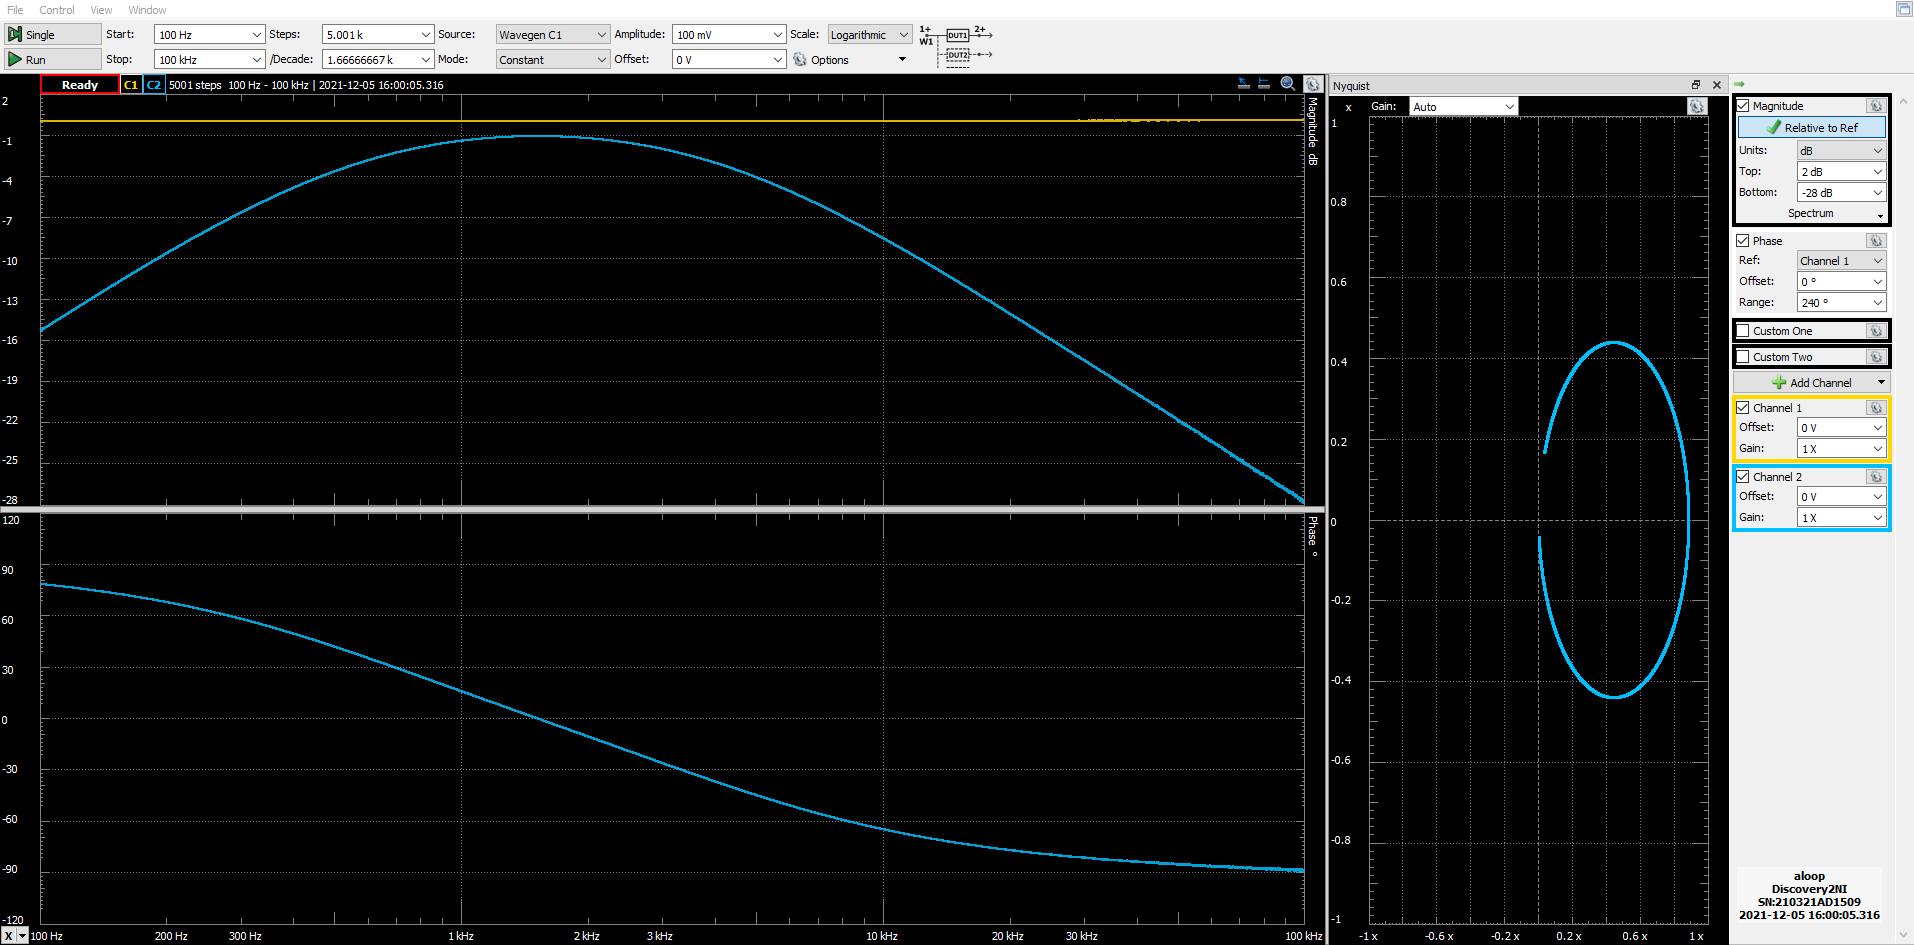
\includegraphics[scale=0.335]{Aloop100Hz}
    \caption{Plot di Bode e Nyquist ottenuto dallo scan con Network tra
    $\SI{100}{\Hz}$ e $\SI{100}{k\Hz}$ con un segnale sinusoidale in ingresso
    all'anello di feedback invertente $A$, di ampiezza costante
    $v\ped{in} = \SI{100}{m\V}$. \label{fig: loopbode}}
\end{figure}

Si è misurata direttamente la frequenza propria dell'oscillatore posizionando
i cursori nel punto in cui la fase si annulla, che corrisponde anche alla
frequenza di centro banda, dove il guadagno della rete di sfasamento è massimo
\begin{align*}
f_0 &= 1522 \pm 2 \; \si{\Hz} \\
A_M &= \abs{\beta(j \omega_0) \bar{A}} =
-1.10 \pm 0.05 \; \si{dB} = 0.881 \pm 0.005
\end{align*}
Inoltre abbiamo ricavato una stima delle frequenze di taglio dal punto in cui
il guadagno diminuisce di $-3.01 \; \si{dB}$ rispetto ad $A_M$
\begin{align*}
f_L &= 804 \pm 2 \; \si{\Hz} \\
f_H &= 2875 \pm 8 \; \si{\Hz}
\end{align*}

\subsection{Dipendenza del loop-gain dalla resistenza del potenziometro}
Riportiamo le misure di massimo e minimo guadagno $A = V\ped{out}/V_s$
trovate al variare della posizione del trimmer:
\begin{align*}
V_s &= 199 \pm 2 \; \si{m\V} \\
V\ped{min} &= 403 \pm 3 \; \si{m\V} \implies  A\ped{v, min} =
2.02 \pm 0.03 \\
V\ped{max} &= 790 \pm 6 \; \si{m\V} \implies  A\ped{v, max} =
3.97 \pm 0.05\\
\end{align*}
questo ci rassicura del fatto che tra i due estremi esista un certo valore di
$p$ per cui il guadagno vale $A(p) = 3$ come richiesto dalla condizione di
auto-oscillazione.

Abbiamo raccolto le nostre misure del guadagno al variare della posizione del
contatto strisciante del potenziometro (o più semplicemente del valore di $p$)
nella \cref{tab: VoutRp}.
\begin{table}[htbp]
\centering
\begin{tabular}{ccccccc}
\toprule
$p$ [arb. un.] & $Rp$ $[\si{\ohm}]$ & $\sigma(Rp)$ & $V\ped{out}$ [mV] &
$\sigma(V\ped{out})$ & $A = V\ped{out}/V_s$ & $\sigma(A)$ \\
\midrule
\midrule
6.3 $\times 10^{-5}$      & 0.6    & 0.2 		& 790    & 6    & 3.97 & 0.05 \\
0.04         & 382		  & 4  	   & 759        & 6      & 3.81 & 0.05 \\
0.10         & 977		  & 8	   & 721        & 6      & 3.62 & 0.05 \\
0.16         & 1550       & 13     & 680        & 5      & 3.42 & 0.04 \\
0.23         & 2.23 k	  & 0.03 k & 642        & 5      & 3.23 & 0.04 \\
0.33         & 3.15 k	  & 0.03 k & 599        & 5      & 3.01 & 0.04 \\
0.43         & 4.09 k	  & 0.04 k & 560        & 4      & 2.81 & 0.04 \\
0.54         & 5.16 k	  & 0.05 k & 520        & 4      & 2.61 & 0.03 \\
0.66         & 6.25 k     & 0.05 k & 483        & 4      & 2.43 & 0.03 \\
0.82         & 7.80 k     & 0.07 k & 442        & 4      & 2.22 & 0.03 \\
1            & 9.53 k     & 0.08 k & 403        & 3      & 2.03 & 0.03 \\  
\bottomrule
\end{tabular}
\caption{Misure di guadagno al variare della tensione in ingresso $V_s$
all'anello di feedback. La forma d'onda in uscita non manifesta difetti
dovuti al clipping dell'op-amp quando questo esce dal regime lineare.
\label{tab: VoutRp}}
\end{table}

\subsubsection{Misure di guadagno al variare di $V_s$}\label{sbs: Vout/Vs}
Misurando con l'oscilloscopio l'ampiezza dei segnali in ingresso $V_s$
e in uscita $v\ped{out}$ dall'amplificatore possiamo ricavare una misura del
guadagno del circuito dal rapporto $A = \dfrac{v\ped{out}}{v\ped{in}}$.

Riportiamo l'andamento qualitativo della forma d'onda in uscita al crescere
dell'ampiezza del segnale in ingresso come visualizzato all'oscilloscopio:

Per un'ampiezza di $V_s = 99.9 \pm 0.8 \; \si{m\V}$ il segnale osservato in
uscita nel dominio dei tempi risulta in buona approssimazione sinusoidale,
riportiamo un fermo immagine dei due segnali studiati come visualizzati
dall'oscilloscopio dell'AD2 in \cref{fig: aloop0.1}
\begin{figure}[htbp]
	\centering
	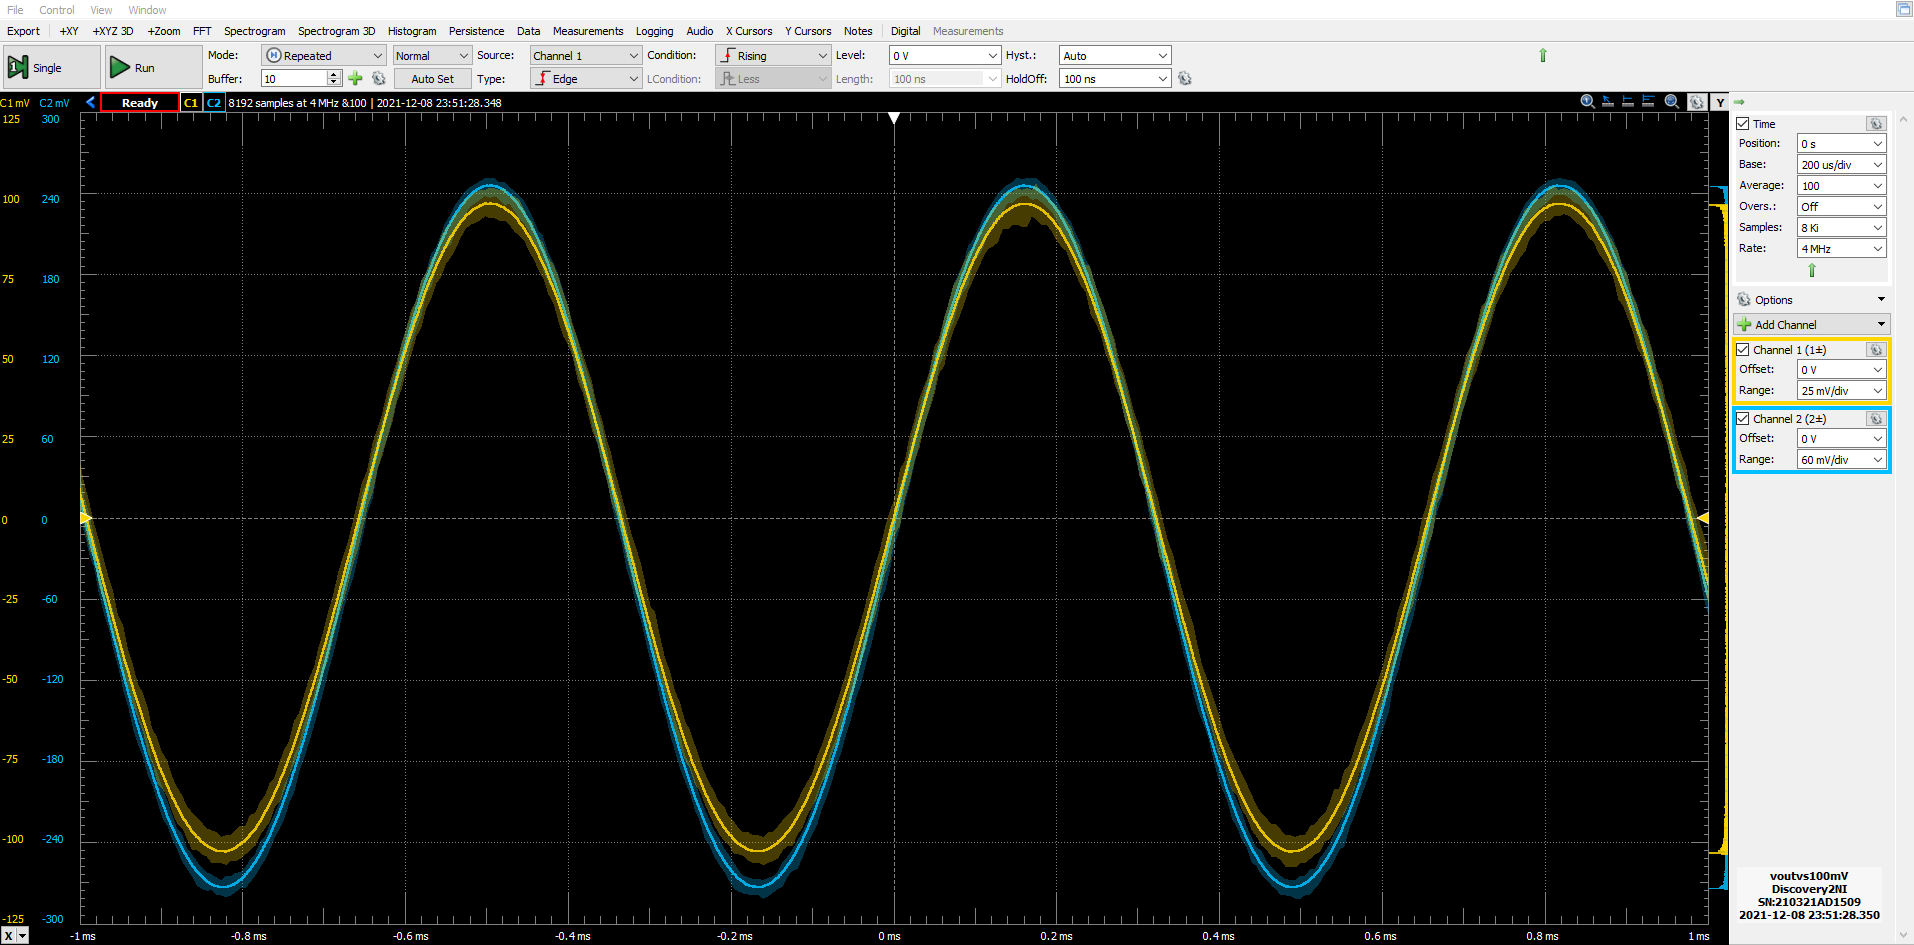
\includegraphics[scale=0.335]{Aloop100mV}
	\caption{Acquisizione presa dall'oscilloscopio dell'andamento nel tempo dei
	segnali $V_s (t)$ (CH1) e $V\ped{out} (t)$ (CH2). \label{fig: aloop0.1}}
\end{figure}

Per ampiezze maggiori dell'onda in ingresso il segnale osservato in uscita
cresce linearmente in ampiezza senza distorsioni apprezzabili, fino a circa
$V_s = 1699 \pm 13 \; \si{m\V}$ per cui la forma d'onda $V\ped{out} (t)$
inizia ad essere affetta da ``clipping'' nel suo semi-periodo negativo
(\cref{fig: aloop1.7}) .
\begin{figure}[htbp]
	\centering
	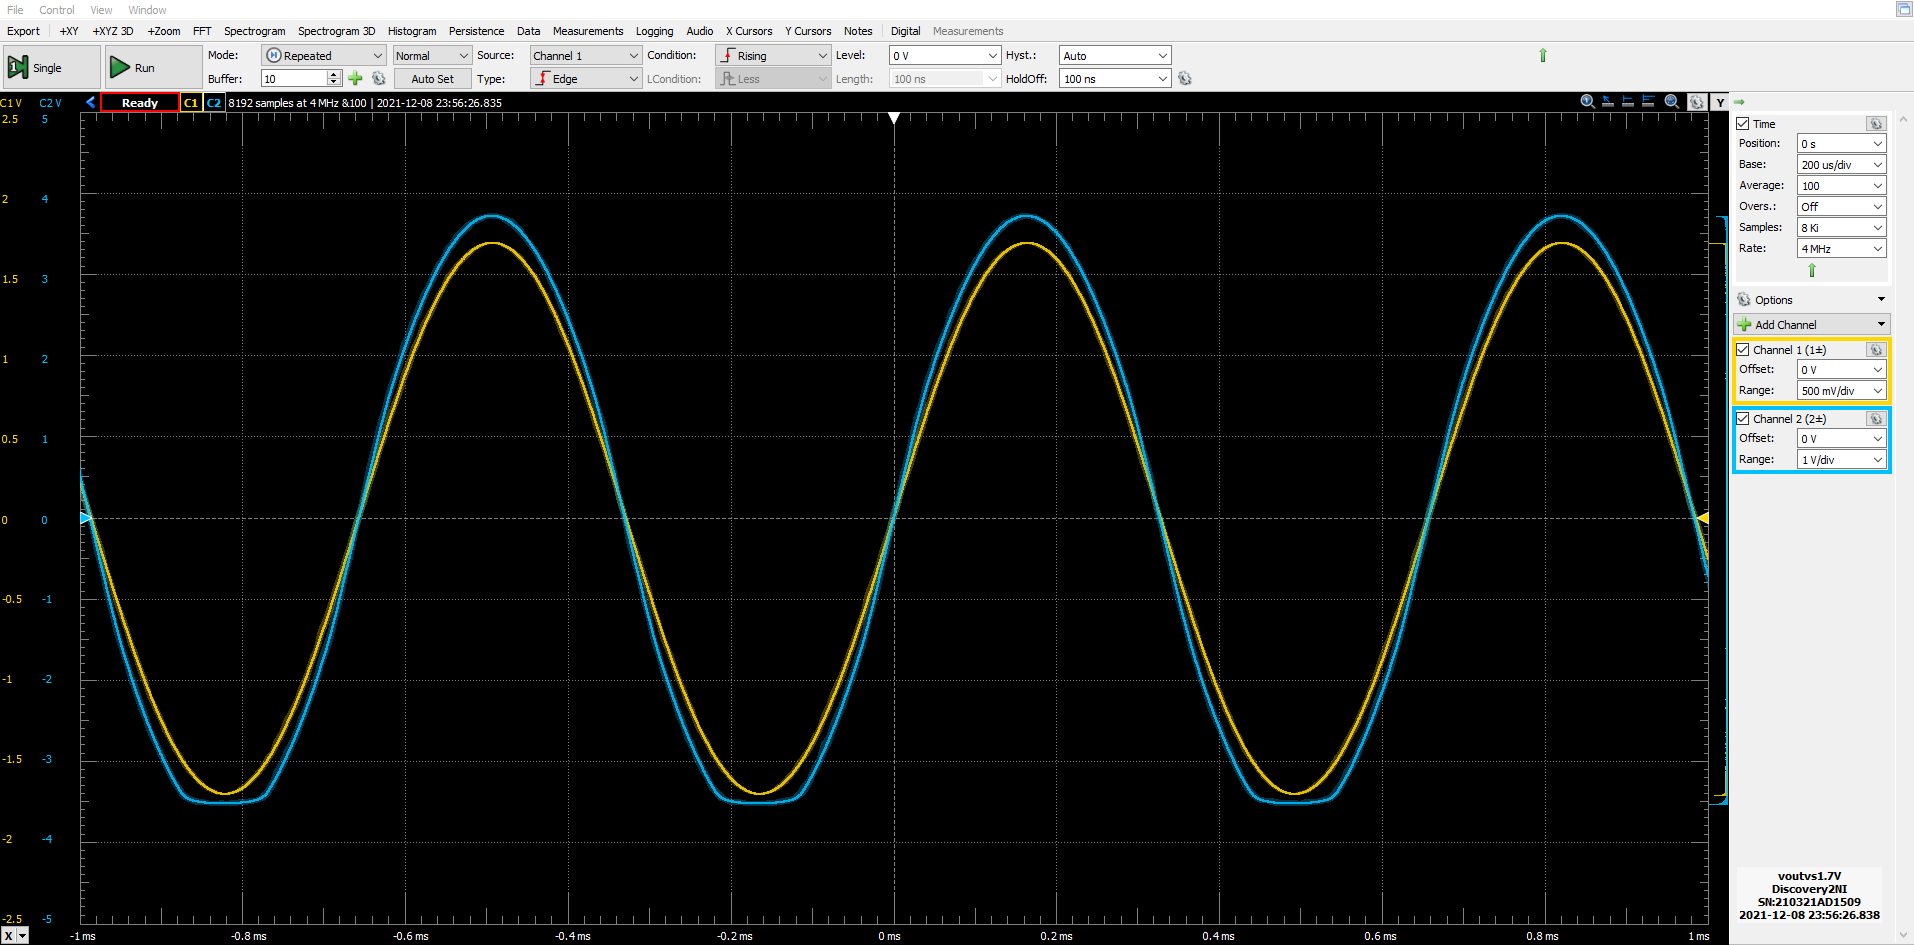
\includegraphics[scale=0.335]{Aloop1.7V}
	\caption{Acquisizione presa dall'oscilloscopio dell'andamento nel tempo dei
	segnali $V_s (t)$ (CH1) e $V\ped{out} (t)$ (CH2). \label{fig: aloop1.7}}
\end{figure}

Continuando ad aumentare l'ampiezza fino a $V_s = 3.01 \pm 0.02 \; \si{\V}$
entrambi i picchi di $V\ped{out} (t)$ vengono tosati alle tensioni di
saturazione positiva e negativa dell'OpAmp (\cref{fig: aloop3}); che quando
abbiamo trattato il Trigger di Schmitt avevamo indicato con
\begin{align*}
V_{OH} &= 4.19 \pm 0.04 \; \si{\V} \\
V_{OL} &= -3.62 \pm 0.03 \; \si{\V}
\end{align*} 
\begin{figure}[htbp]
	\centering
	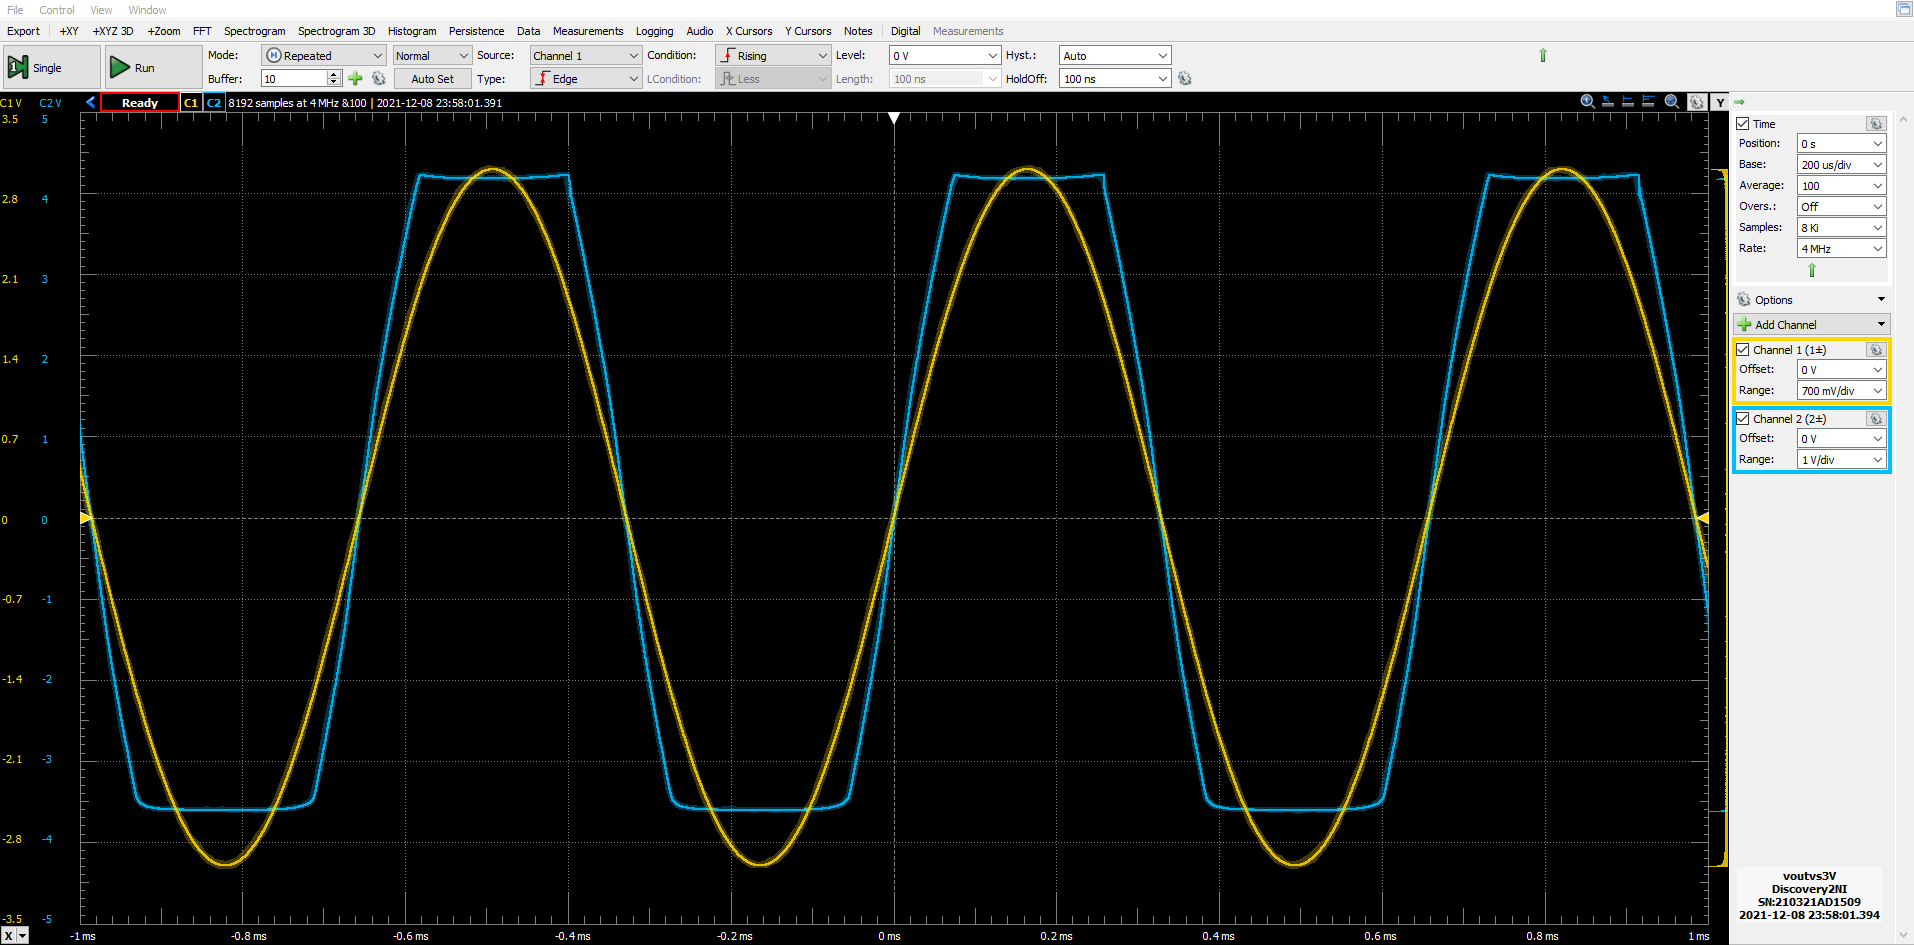
\includegraphics[scale=0.335]{Aloop3V}
	\caption{Acquisizione presa dall'oscilloscopio dell'andamento nel tempo dei
	segnali $V_s (t)$ (CH1) e $V\ped{out} (t)$ (CH2). \label{fig: aloop3}}
\end{figure}

Infine, quando l'ampiezza in ingresso supera $V_{OH}$ osserviamo l'onda quadra
in uscita commutare livello due volte nello stesso periodo, proprio in
corrispondenza del passaggio di $V_s (t)$ dalle tensioni di saturazione del
TL081 (\cref{fig: aloop4.5}).
\begin{figure}[htbp]
	\centering
	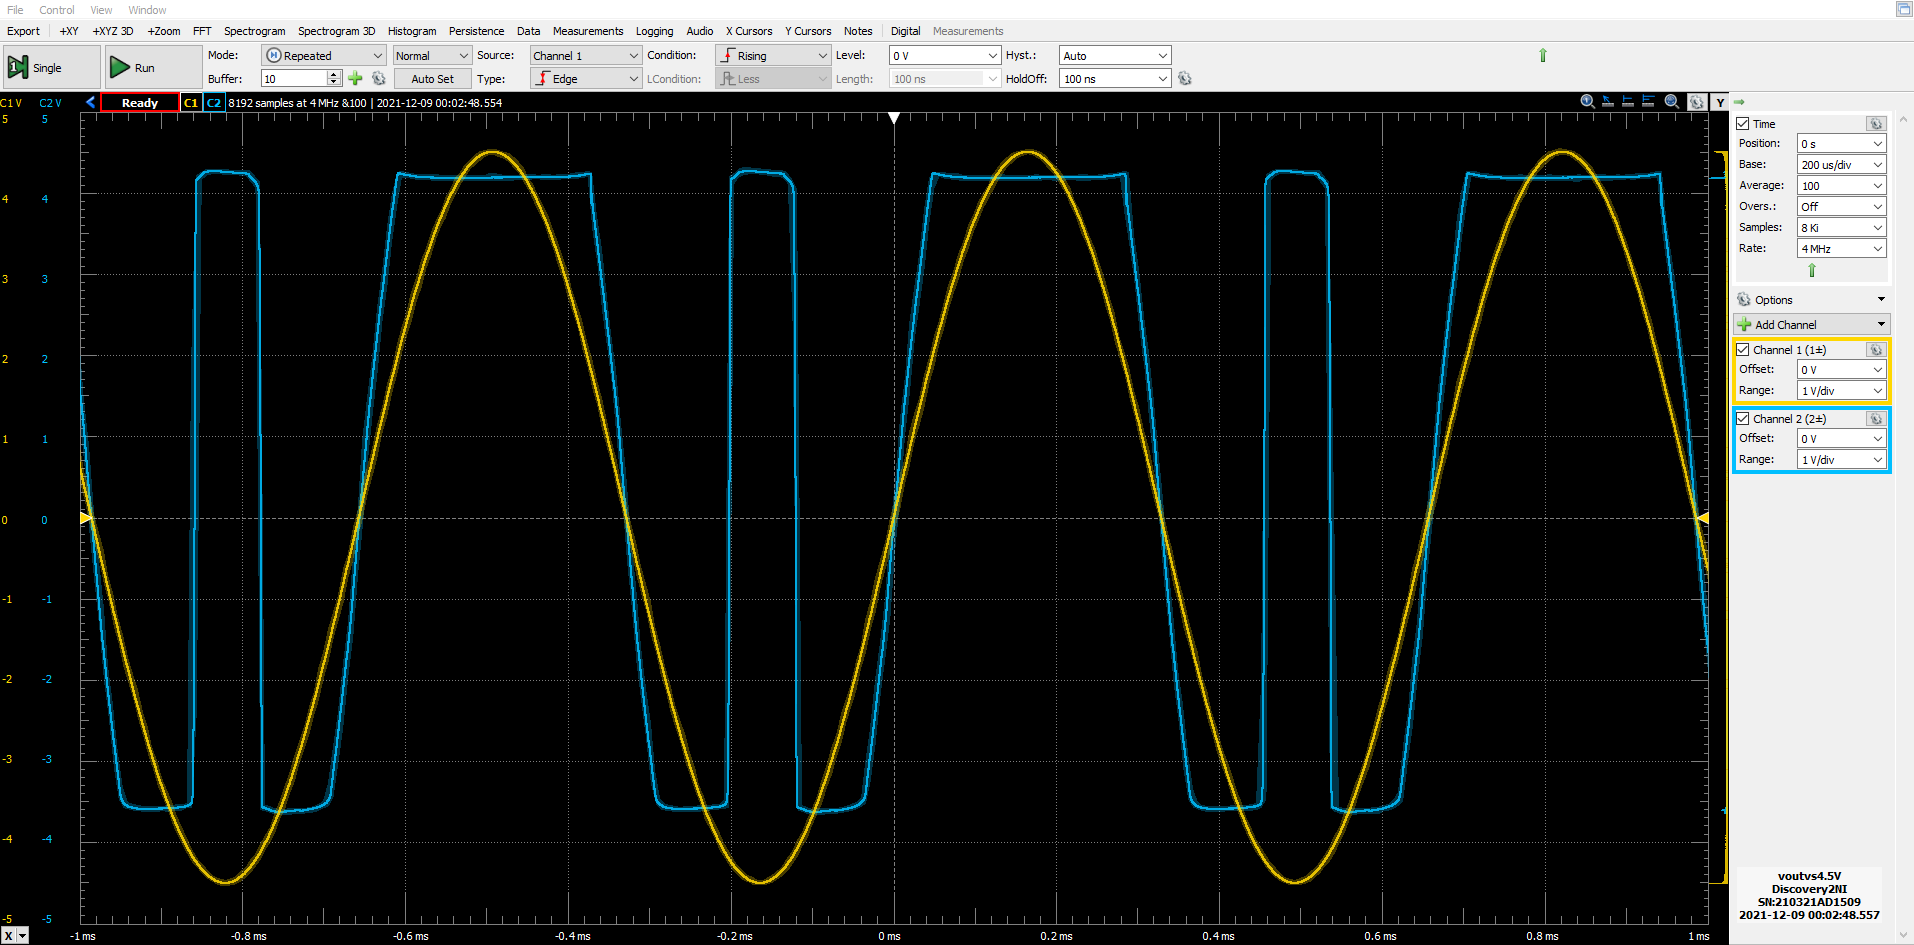
\includegraphics[scale=0.335]{Aloop4.5V}
	\caption{Acquisizione presa dall'oscilloscopio dell'andamento nel tempo dei
	segnali $V_s (t)$ (CH1) e $V\ped{out} (t)$ (CH2). \label{fig: aloop4.5}}
\end{figure}

Con un fit lineare possiamo stimare il guadagno dell'amplificatore a partire
dal grafico di $v\ped{out} = A v\ped{in}$ al variare di $v\ped{in}$.
Riportiamo quanto trovato per il primo circuito:
\begin{figure}[htbp]
\centering
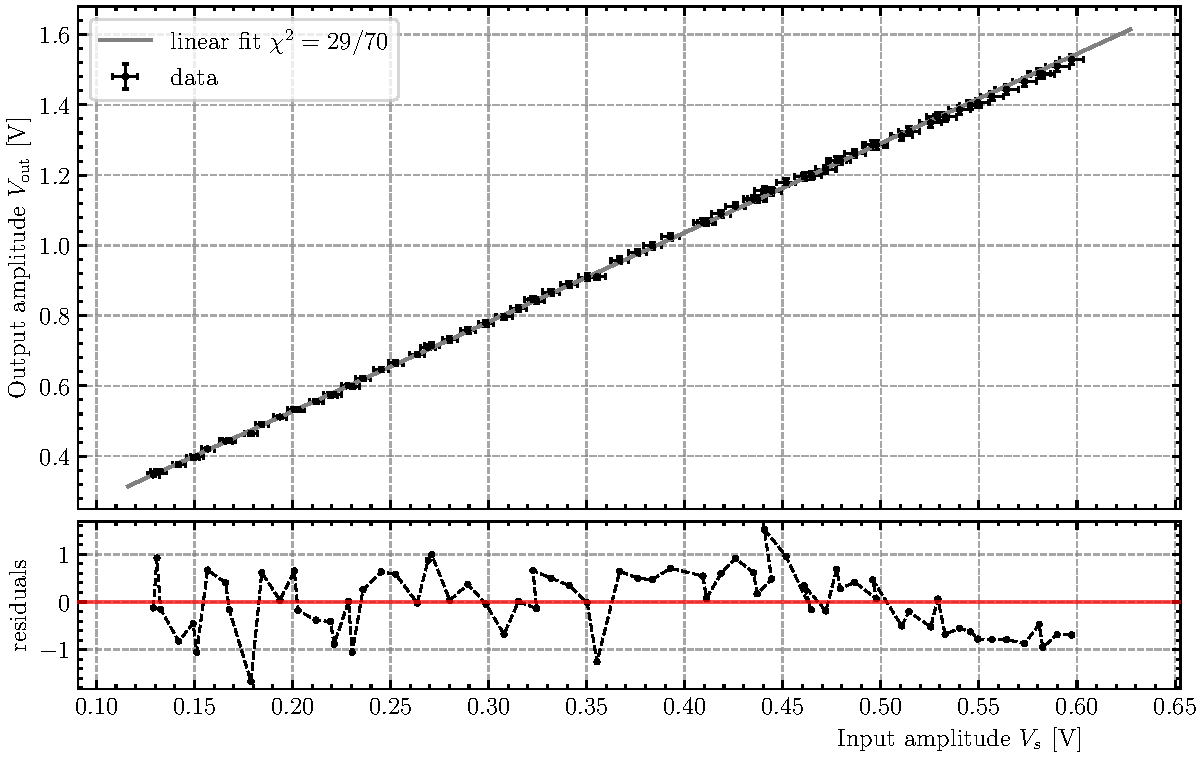
\includegraphics[scale=0.7]{gainfit}
\caption{Fit lineare per l'andamento dell'ampiezza misurata in uscita rispetto
all'ampiezza del segnale in ingresso. \label{fig: gainfit}}
\end{figure}
Da cui troviamo i seguenti parametri per la retta di best-fit
\begin{align*}
\text{intercetta} = 18.7 \pm 1.3 \; \si{m\V} \;\;\;
\text{pendenza} = 2.544 \pm 0.004 \;\;\; \text{correlazione} = -0.90
\;\;\; \chi^2 = 29 \;\;\; \text{d.o.f.} = 70
\end{align*}

Il valore atteso per il guadagno calcolato a partire dal valore dei componenti
in questa configurazione del circuito
($Rp = 5.43 \pm 0.05 \; \si{k\ohm} \implies p = 0.570 \pm 0.007$)
è data dalla \cref{eq: A}
\[
A\ped{exp} = \frac{R + R_3 + R_4 + R_5}{Rp + R_5} = 2.55 \pm 0.03
\]
Questo è in ottimo accordo con quanto trovato sperimentalmente dalla nostra
analisi.

Per completezza riportiamo in \cref{fig: gainsat} anche le misure che non
abbiamo considerato nel fit perché oltre la regione in cui l'op-amp ha
comportamento lineare
\begin{figure}[htbp]
\centering
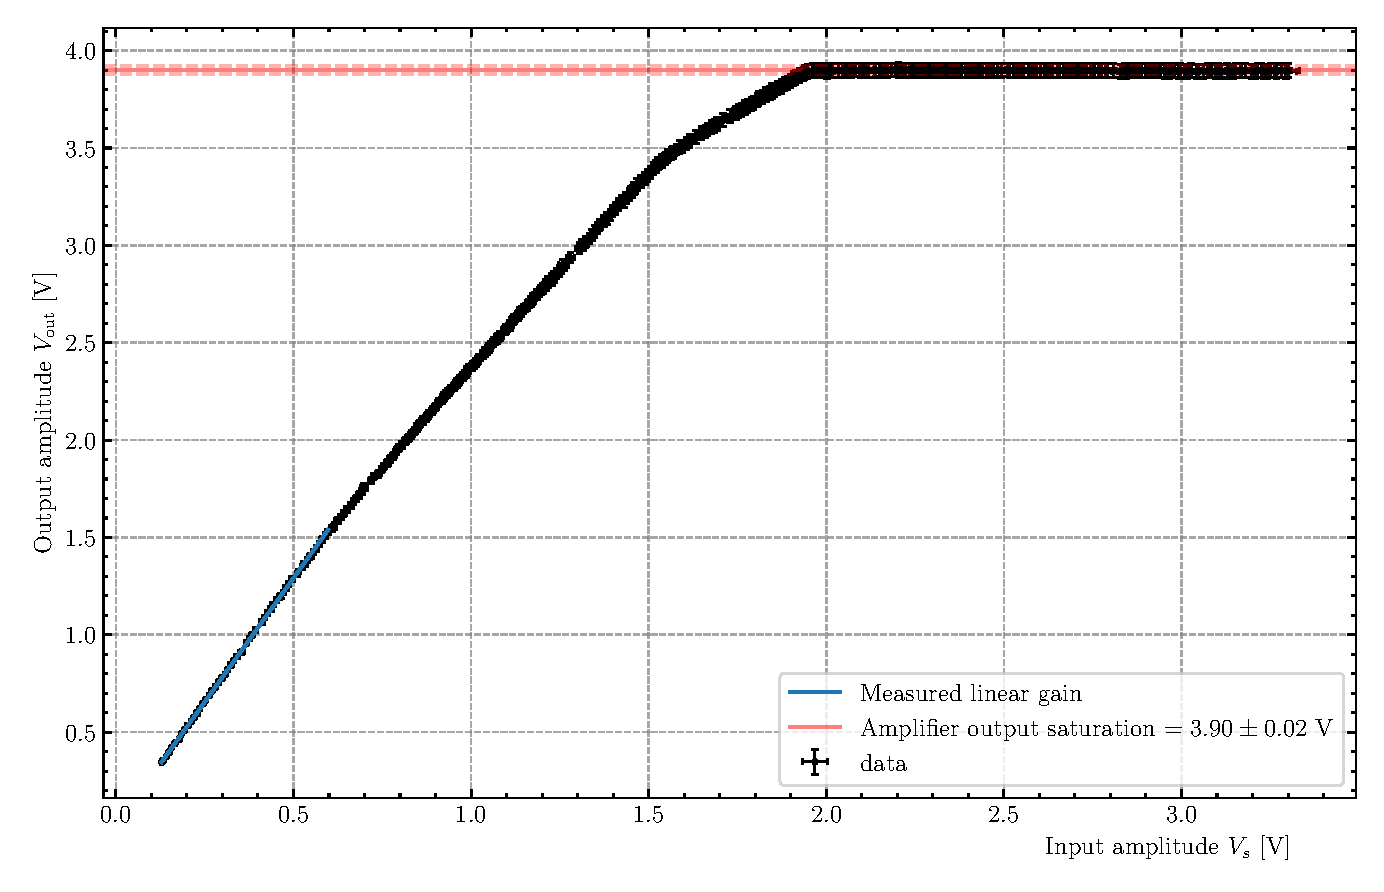
\includegraphics[scale=0.7]{VoutVs}
\caption{Andamento reale dell'ampiezza del segnale in uscita al variare
dell'ampiezza del segnale in ingresso, anche oltre il regime lineare
dell'amplificatore. \label{fig: gainsat}}
\end{figure}

%=======================
\section{Progettazione del circuito auto-oscillante}
Si è completato il circuito oscillatore a ponte di Wien collegando
l'ingresso non-invertente dell'OpAmp TL081CP al punto A, quindi chiudendo
l'anello di feedback positivo, come si vede in \cref{fig: wienschm}
\begin{figure}[htbp]
    \centering
	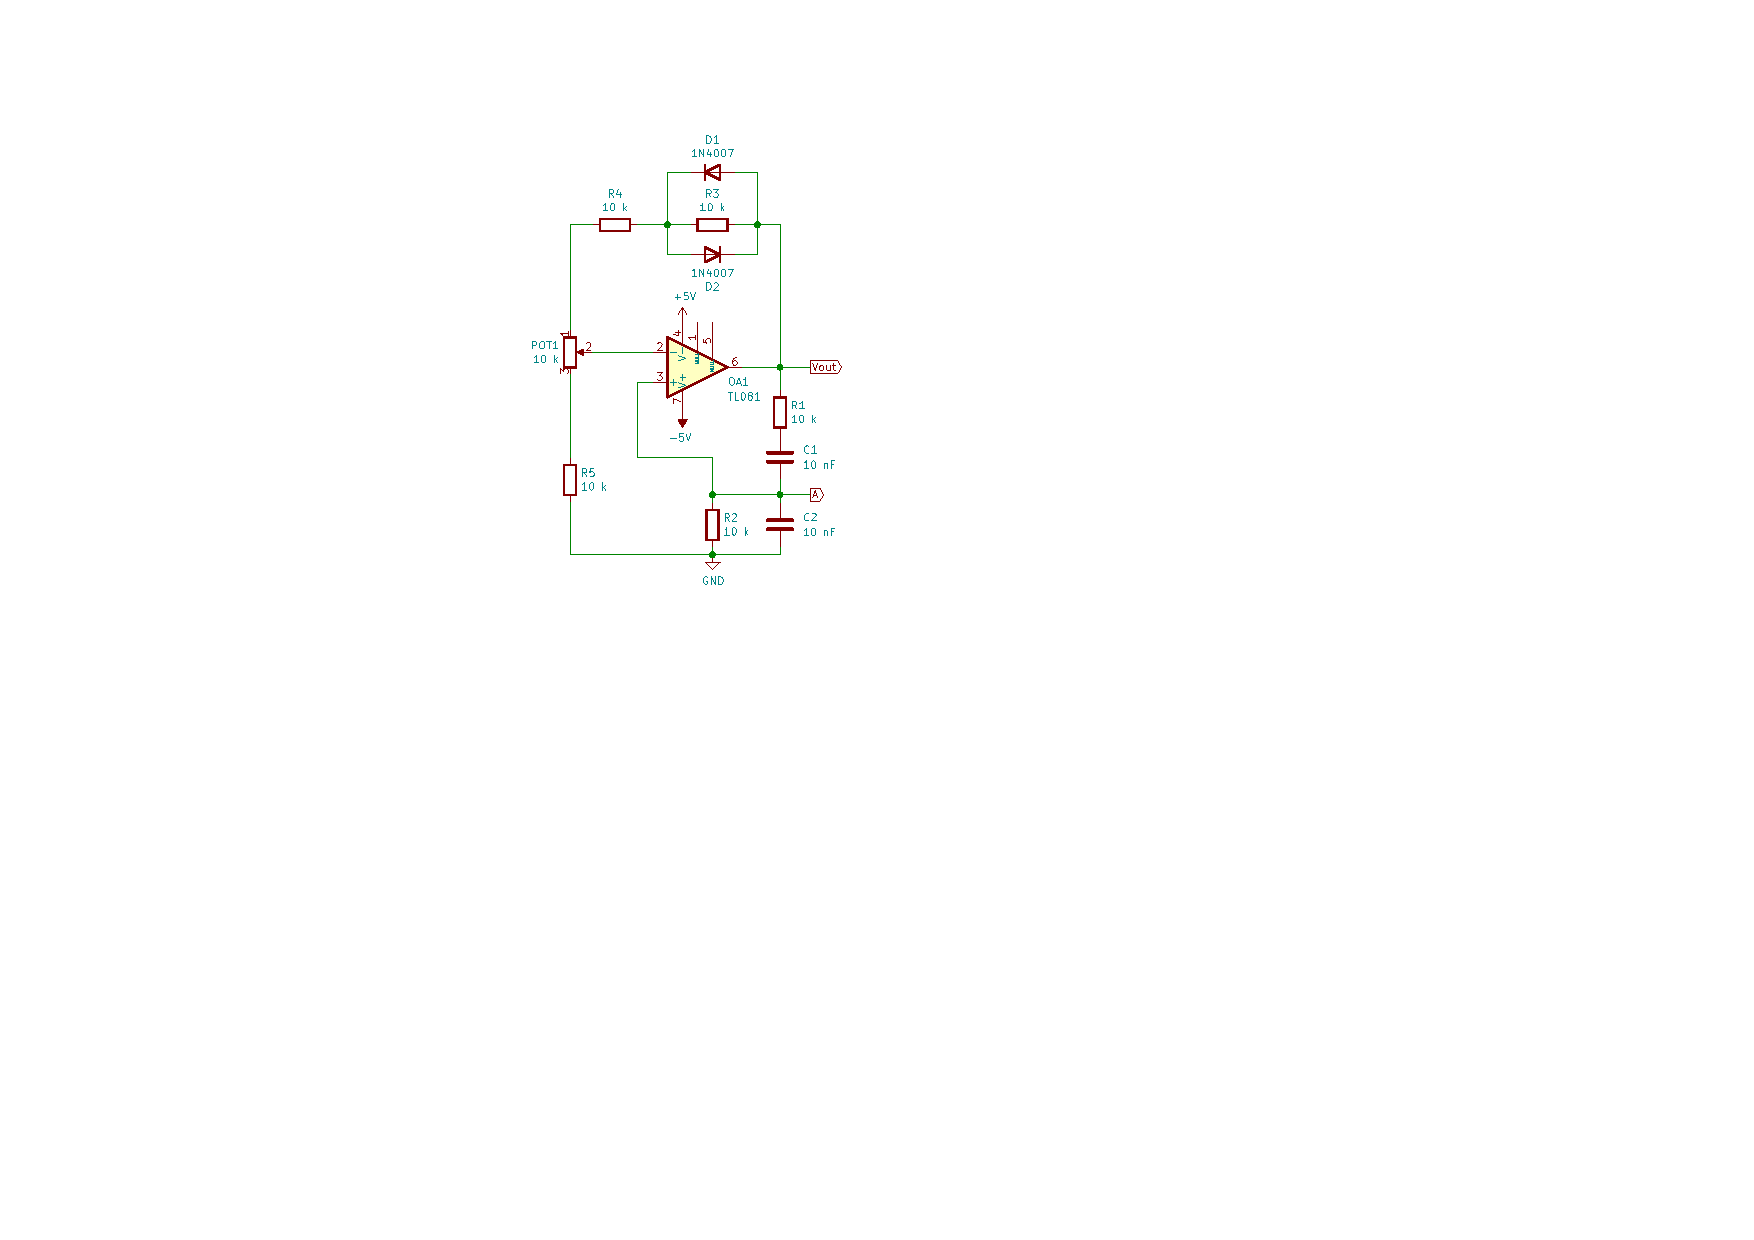
\includegraphics[scale=1.2]{wienschm}
    \caption{Schema circuitale dell'oscillatore a ponte di Wien studiato.
    \label{fig: wienschm}}
\end{figure}

%=======================
\section{Frequenza generata e innesco dell'oscillazione}
\subsection{Misura della frequenza generata dall'oscillatore}
Per il valore massimo della resistenza del potenziometro per cui osserviamo
un segnale oscillante in uscita dal circuito
$Rp\ped{max} = 2.96 \pm 0.03 \; \si{k\ohm}$ abbiamo misurato la frequenza del
segnale con tre metodi diversi:
Come prima stima della frequenza propria dell'oscillatore abbiamo preso la
frequenza in cui si osserva l'unico picco presente nella FFT del segnale
$v\ped{out} (t)$ determinata con l'uso dei cursori
\[
f_0 = 1.52 \pm 0.02 \; \si{k\Hz}
\]
Tramite la funzione di misura automatica ``Measurements > frequency''
dell'AD2
\[
f_0 = 1517 \pm 15 \; \si{\Hz}
\]
Perfettamente compatibile con una misura diretta del periodo del segnale nel
dominio dei tempi, fatta sempre utilizzando i cursori
\begin{align*}
T_0 &= 660 \pm 8 \\
f_0 &= 1516 \pm 18 \; \si{\Hz}
\end{align*}

\begin{figure}[htbp]
	\centering
	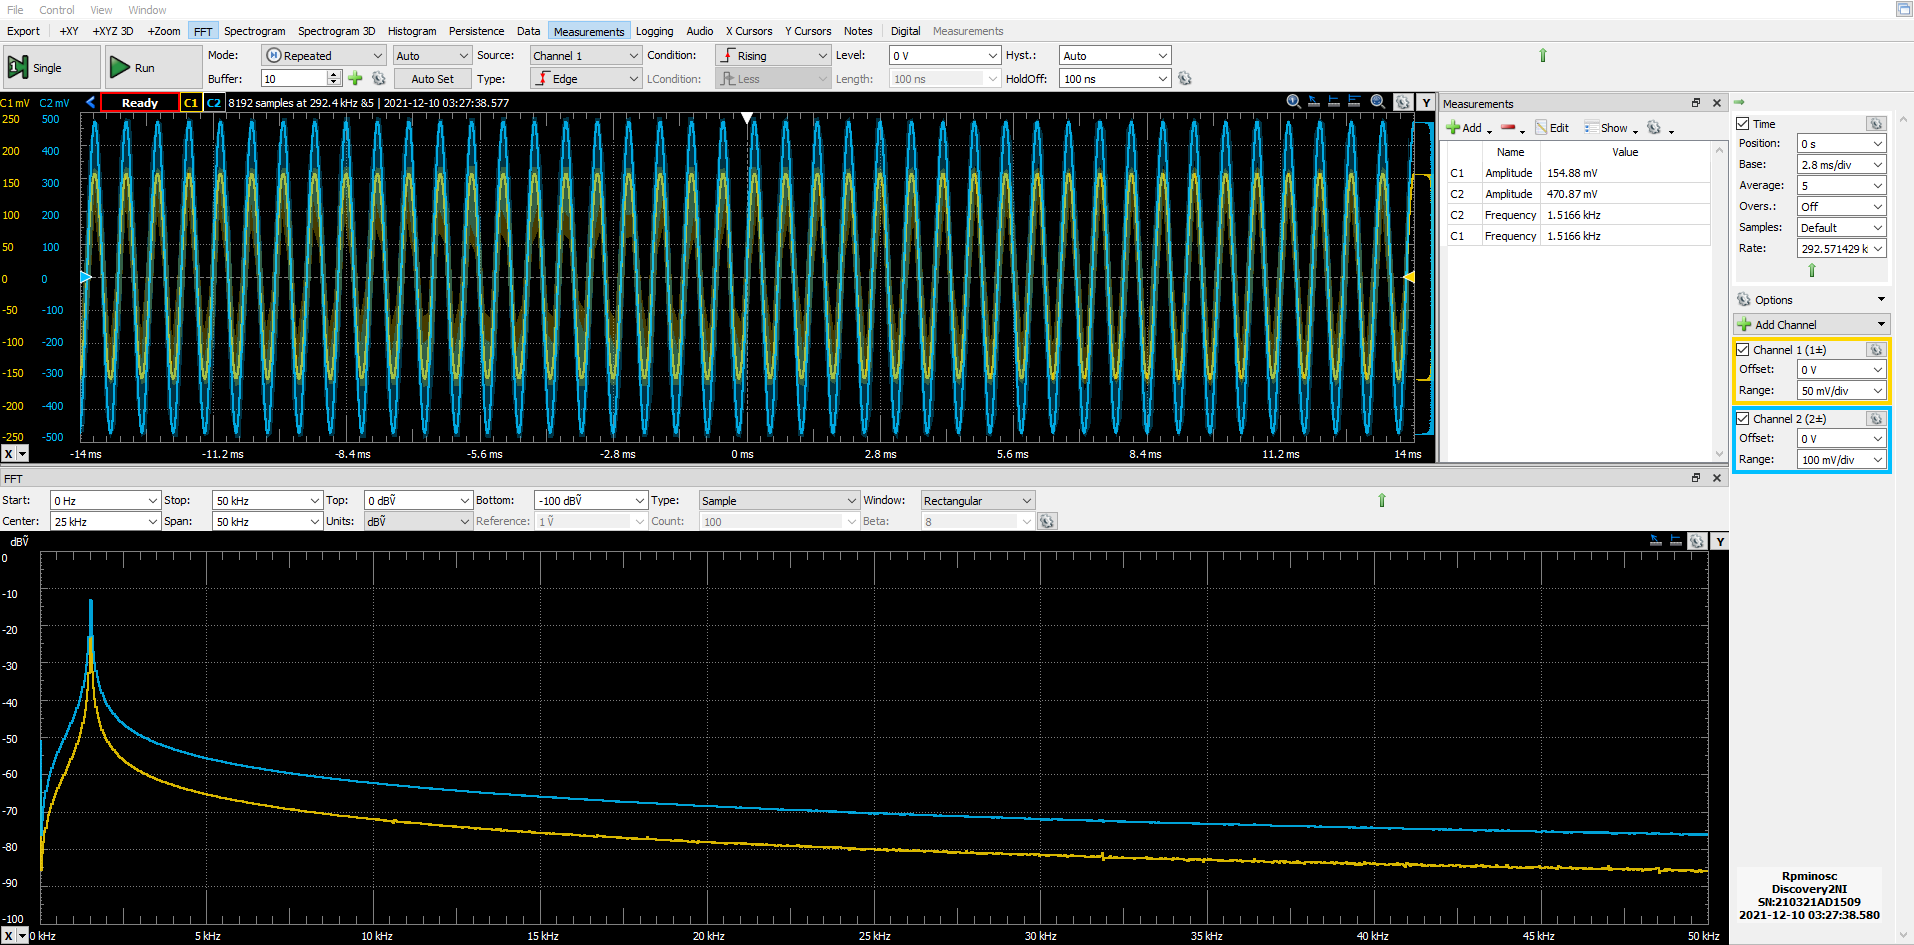
\includegraphics[scale=0.335]{Rpminosc}
	\caption{Fermo immagine preso dall'oscilloscopio per illustrare i tre
	metodi di misura sperimentati. Le tracce dei segnali corrispondono a
	$v_+ (t)$ (CH1) e $v\ped{out} (t)$ (CH2). Dalle trasformate di Fourier dei
	segnali non si riescono ad apprezzare armoniche superiori alla fondamentale
	 \label{fig: Rpmin}}
\end{figure}

Tutti e tre i metodi forniscono misure compatibili con il valore atteso
\begin{equation}\label{eq: f0exp}
f_0 = \frac{1}{2 \pi \sqrt{R_1 C_1 R_2 C_2}} = 1.53 \pm 0.06 \; \si{k\Hz}
\end{equation}

\subsection{Dipendenze dalla posizione del potenziometro}
Al variare del parametro $p$ del potenziometro si evidenziano tre principali
regimi di operazione del circuito:
\begin{description}
\item[$1 < p < p\ped{max}$]
dove in uscita dall'OpAmp non si riesce ad osservare il segnale sinusoidale
che intendiamo generare. In questa configurazione qualsiasi segnale viene
attenuato dal circuito fino a non essere distinguibile dal rumore di fondo
dello strumento.
\item[$p\ped{max} < p < p\ped{dist}$]\label{item: posc}
dove il segnale in uscita $V\ped{out} (t)$ è in buona approssimazione
una sinusoide con frequenza prossima a quella propria dell'oscillatore $f_0$.
In questa configurazione il guadagno del circuito è sufficiente per sostenere
l'oscillazione sinusoidale in maniera stabile senza che l'uscita del circuito
diverga fino alla saturazione.
\item[$p\ped{dist} < p < 0$]
dove $V\ped{out} (t)$ mostra significative distorsioni non lineari dovute alla
presenza dei diodi e dalla potenza finita che il TL081 è in grado di erogare.
In questa configurazione il guadagno dell'anello amplificatore tende a
divergere, quindi qualsiasi segnale cresce in ampiezza fino a raggiungere la
saturazione dell'OpAmp.
\end{description}

In corrispondenza del valore massimo di $p$ per cui riusciamo ad osservare un
seno in uscita dall'oscillatore abbiamo misurato il valore minimo assunto
dall'ampiezza del segnale in uscita $V\ped{out, min} = 471 \pm 4 \; \si{m\V}$
alla sua frequenza massima di $f\ped{max} = 1516.2 \pm \; \si{\Hz}$
(compatibile con il valore misurato di $f_0$)

Al decrescere della resistenza $Rp$ si vede che l'ampiezza aumenta fino ad
un'ampiezza picco-picco massima di $V\ped{out, max} = 7.78 \pm 0.04 \; \si{\V}$
(compatibile con la differenza tra le tensioni di saturazione positiva e
negativa $V_{OH} - V_{OL} = 7.81 \pm 0.05 \; \si{\V}$), mentre
la frequenza dell'onda diminuisce fino al valore minimo osservato di
$f\ped{min} = 1423.4 \; \si{\Hz}$.

Osservando il segnale in uscita $V\ped{out} (t)$ ci si aspetta di trovare
un'onda sinusoidale di ampiezza picco-picco massima $\sim \SI{8}{\V}$ e
frequenza dello stesso ordine di grandezza di quella propria dell'oscillatore
$f_0$, vista in \cref{eq: f0exp}.
Mentre come $v_+ (t) = V_A (t)$ ci aspettiamo un'onda della stessa forma di
$v\ped{out} (t) = A(p) v_+ (t)$, ma ridotta in ampiezza dalla funzione di
trasferimento reale $1/A$ e lo stesso segnale all'ingresso negativo.

Questo corrisponde all'andamento osservato dei segnali, che riportiamo
nelle seguenti figure al variare della frazione di resistenza del
potenziometro $p$. 

Per un valore di resistenza pari a
$Rp\ped{dist} = 2.17 \pm 0.03 \; \si{k\ohm} \implies p = 0.228 \pm 0.004$ 
abbiamo come fattore di riscalamento $1/A = 0.308 \pm 0.003$
e si iniziano a notare le distorsioni dell'onda in uscita rispetto ad una
sinusoide (\cref{fig: Rpdist}).
\begin{figure}[htbp]
	\begin{center}
	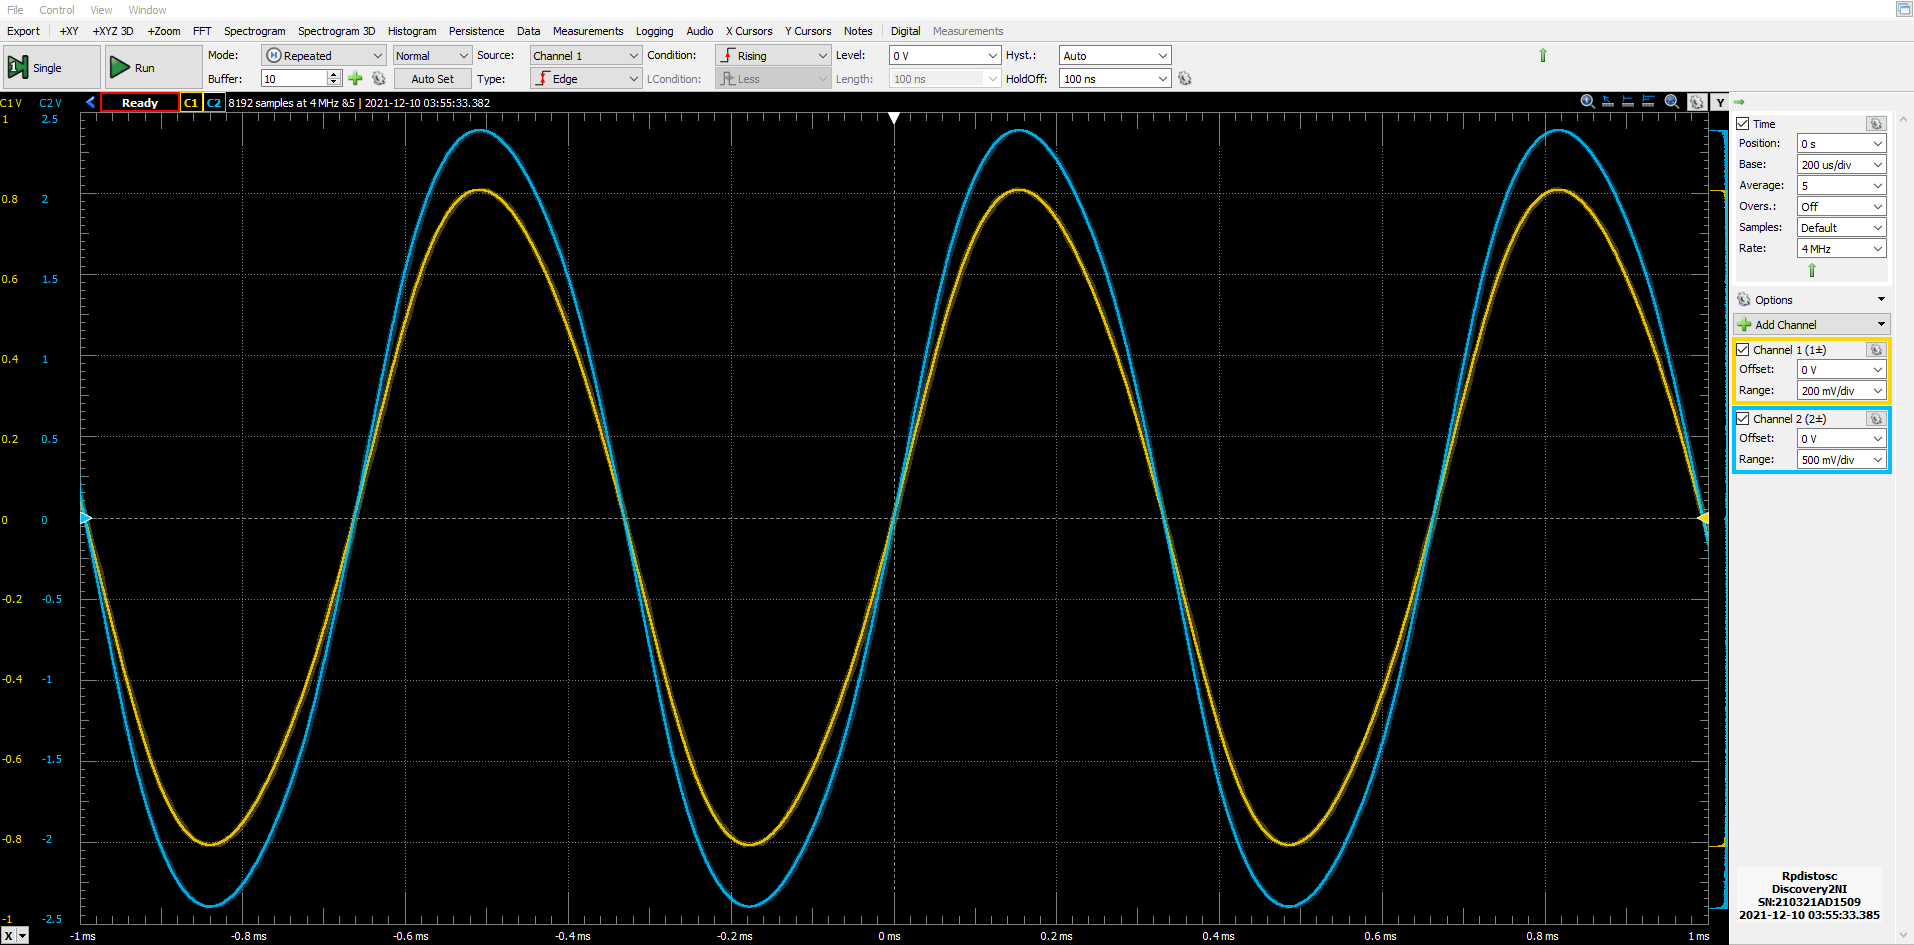
\includegraphics[width=\textwidth]{Rpdistosc800mV}
	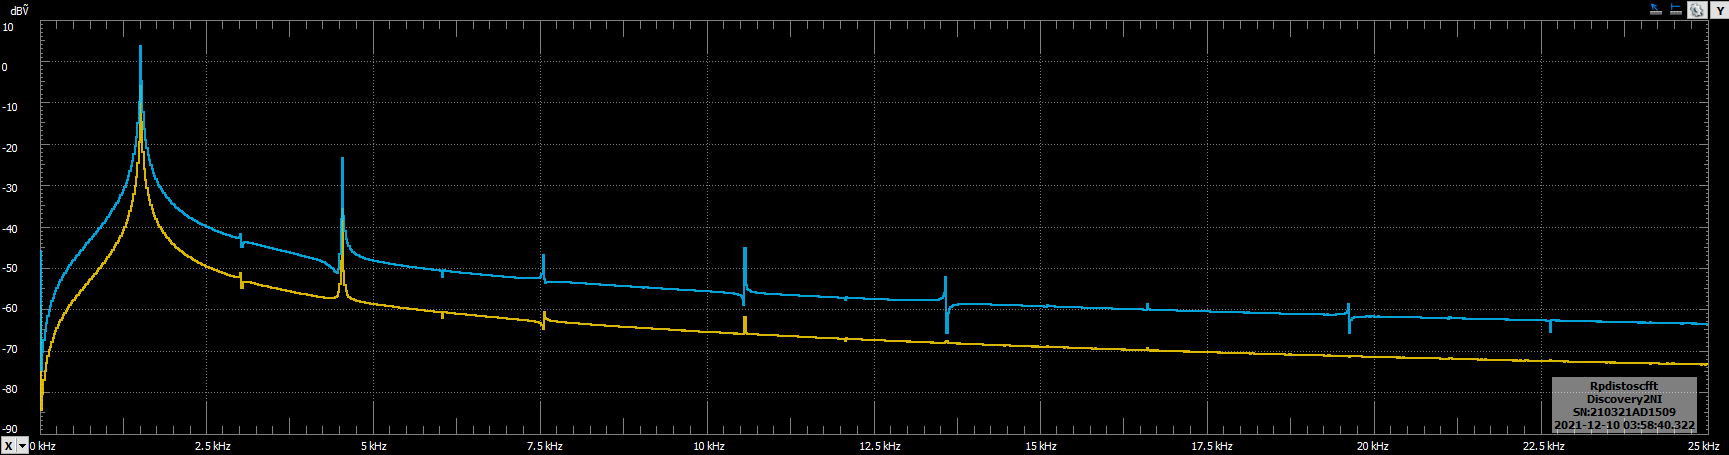
\includegraphics[width=\textwidth]{Rpdistosc800mVfft}
	\caption{Fermo immagine preso dall'oscilloscopio dell'andamento nel tempo dei
	segnali $v_+ (t)$ (CH1) e $V\ped{out} (t)$ (CH2). Nelle FFT dei segnali si
	nota bene la presenza di armoniche spurie multiple della fondamentale $f_0$.
	\label{fig: Rpdist}}
	\end{center}
\end{figure}

Dunque per
$Rp\ped{int} = 1454 \pm 12 \; \si{\ohm} \implies p = 0.153 \pm 0.002$ 
abbiamo come fattore di riscalamento $1/A = 0.290 \pm 0.003$; in particolare
la forma d'onda in uscita ora ha semiperiodo negativo tagliato a
$V_{OL} \approx 3.5 \; \si{\V}$ in maniera simile al regime di interdizione
visto per un amplificatore con BJT a emettitore comune (\cref{fig: Rpint}).
\begin{figure}[htbp]
	\centering
	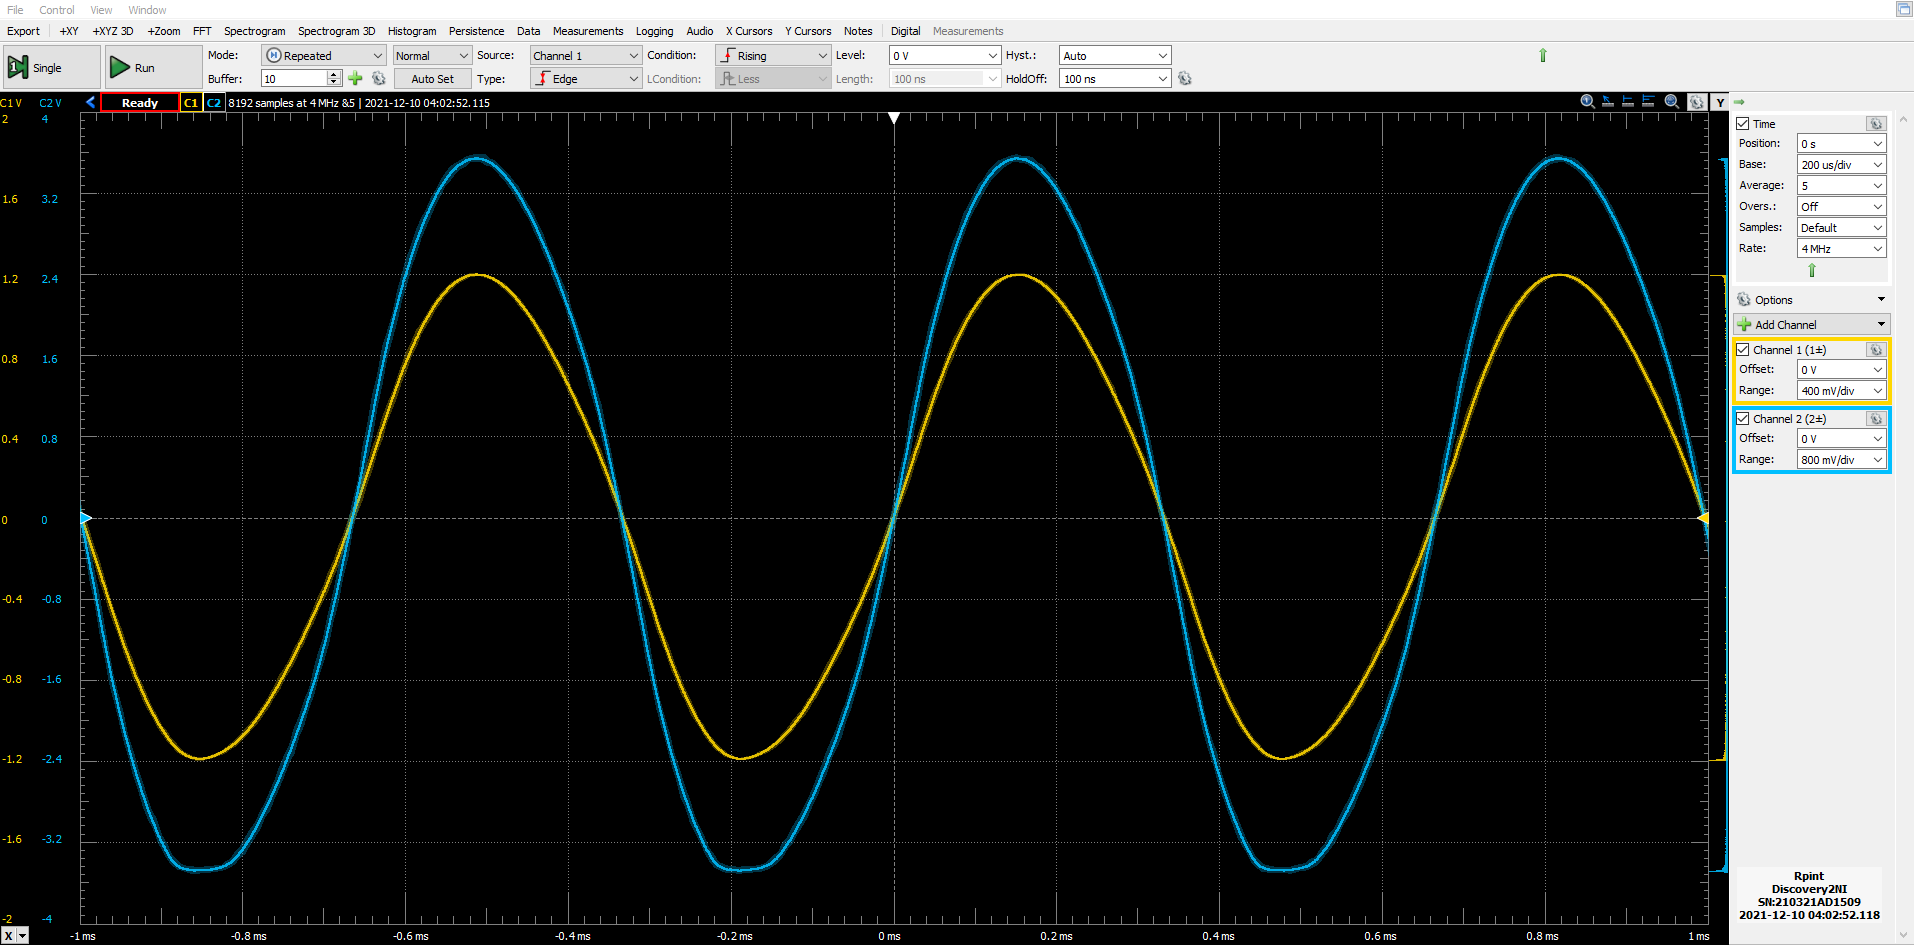
\includegraphics[width=\textwidth, height=.25\paperheight]{Rpint1.2V}	
	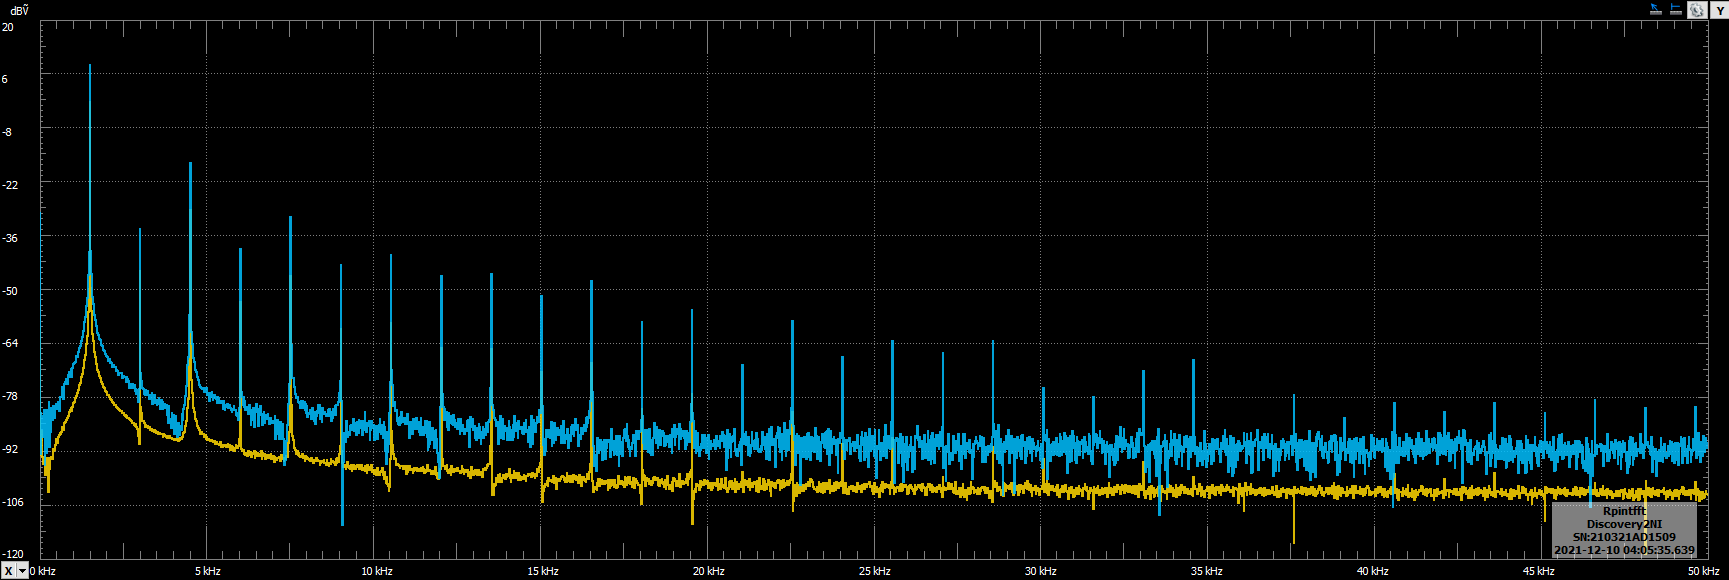
\includegraphics[width=\textwidth]{Rpint1.2Vfft}
	\caption{Fermo immagine preso dall'oscilloscopio dell'andamento nel tempo dei
	segnali $v_+ (t)$ (CH1) e $V\ped{out}$ (CH2). Dalle trasformate di Fourier
	(di sotto) si nota un significativo aumento nel numero di picchi, a ulteriore
	conferma del fatto che non ci troviamo più in regime lineare.
	\label{fig: Rpint}}
\end{figure}

Spostando il contatto strisciante fino al minimo valore del potenziometro
la forma d'onda in uscita risulta affetta da clipping in entrambi i semiperiodi
del segnale; inoltre per
$Rp = 2.3 \pm 0.2 \; \si{k\ohm} \implies p = (2.4 \pm 0.8) \times 10^{-4}$ 
abbiamo come fattore di riscalamento $1/A \approx 0.253 \pm 0.003$
(\cref{fig: Rpmax}).
\begin{figure}[htbp]
	\centering
	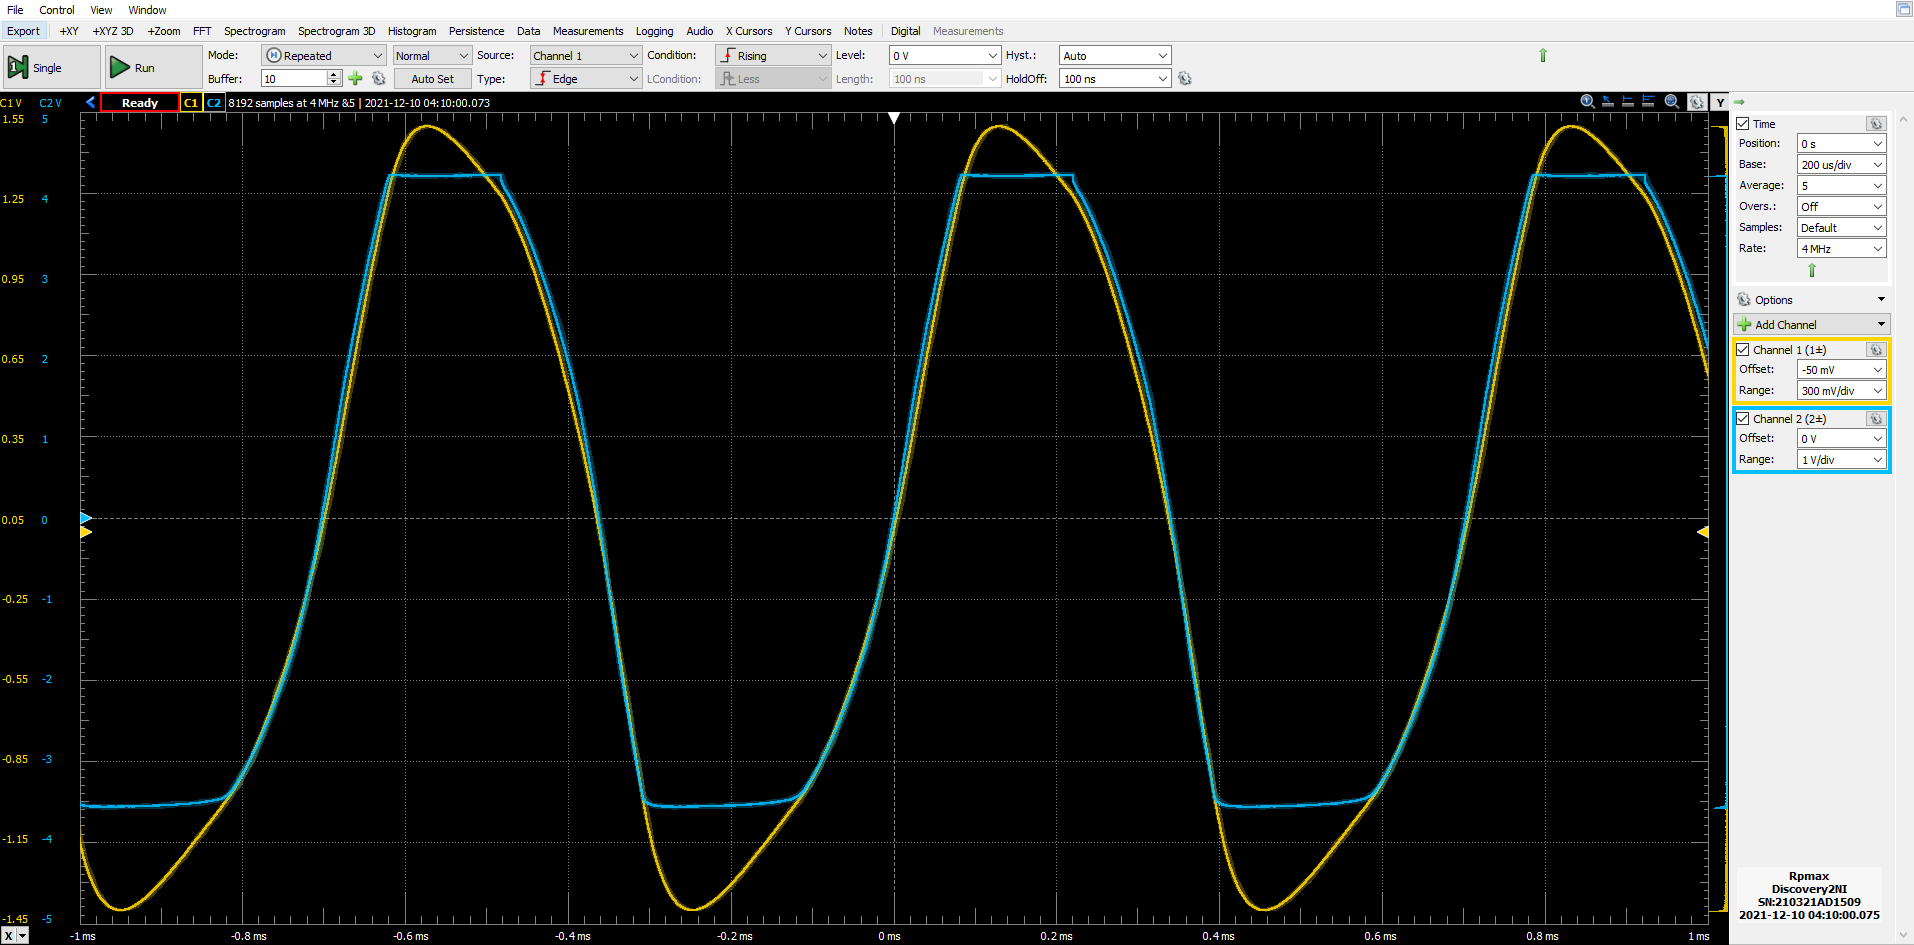
\includegraphics[width=\textwidth, height=.25\paperheight]{Rpmax1.5V}
	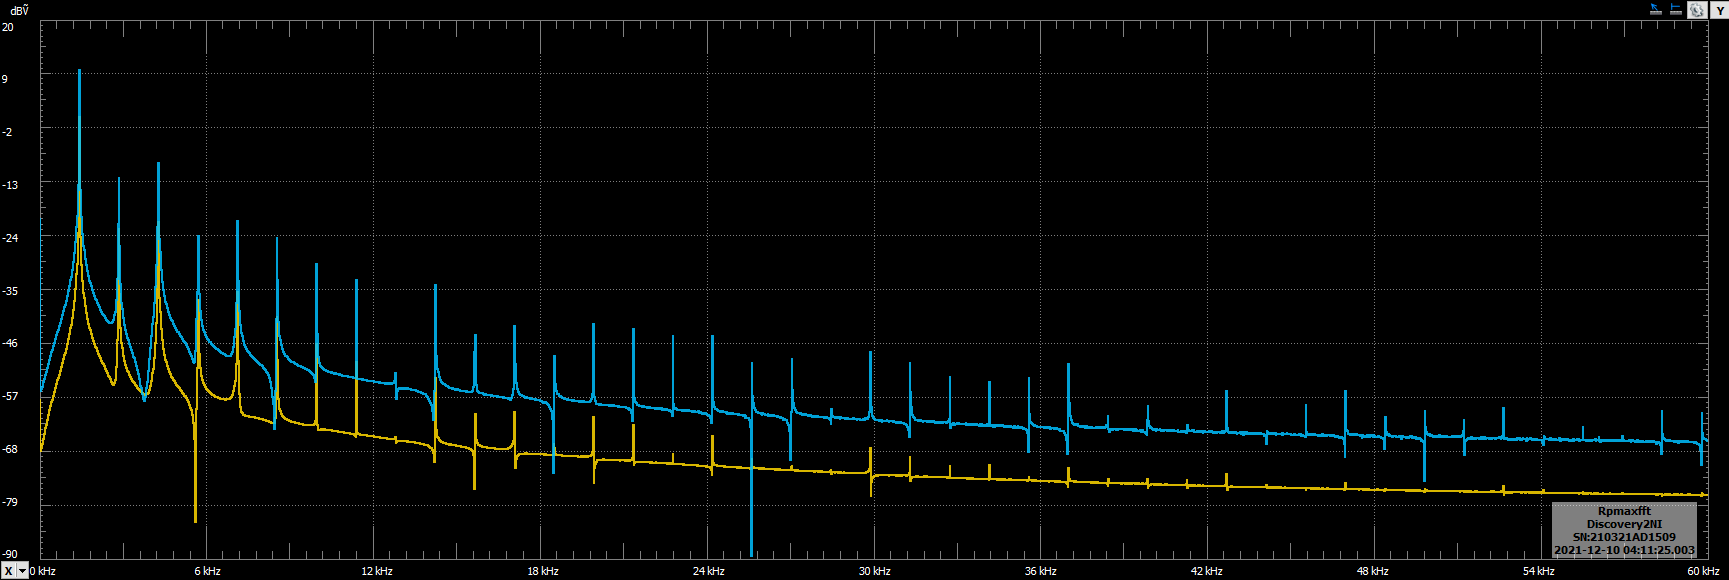
\includegraphics[width=\textwidth]{Rpmax1.5Vfft}
	\caption{Fermo immagine preso dall'oscilloscopio dell'andamento nel tempo dei
	segnali $v_+ (t)$ (CH1) e $V\ped{out} (t)$ (CH2) e relative trasformate di
	Fourier. \label{fig: Rpmax}}
\end{figure}

\subsection{Innesco dell'auto-oscillazione}
Mettendo in corto-circuito il parallelo di $R_3$ con i diodi si riesce a
bloccare l'oscillazione del segnale in uscita dal circuito, come si vede in
\cref{fig: Rpminstop}.
\begin{figure}[htbp]
	\centering
	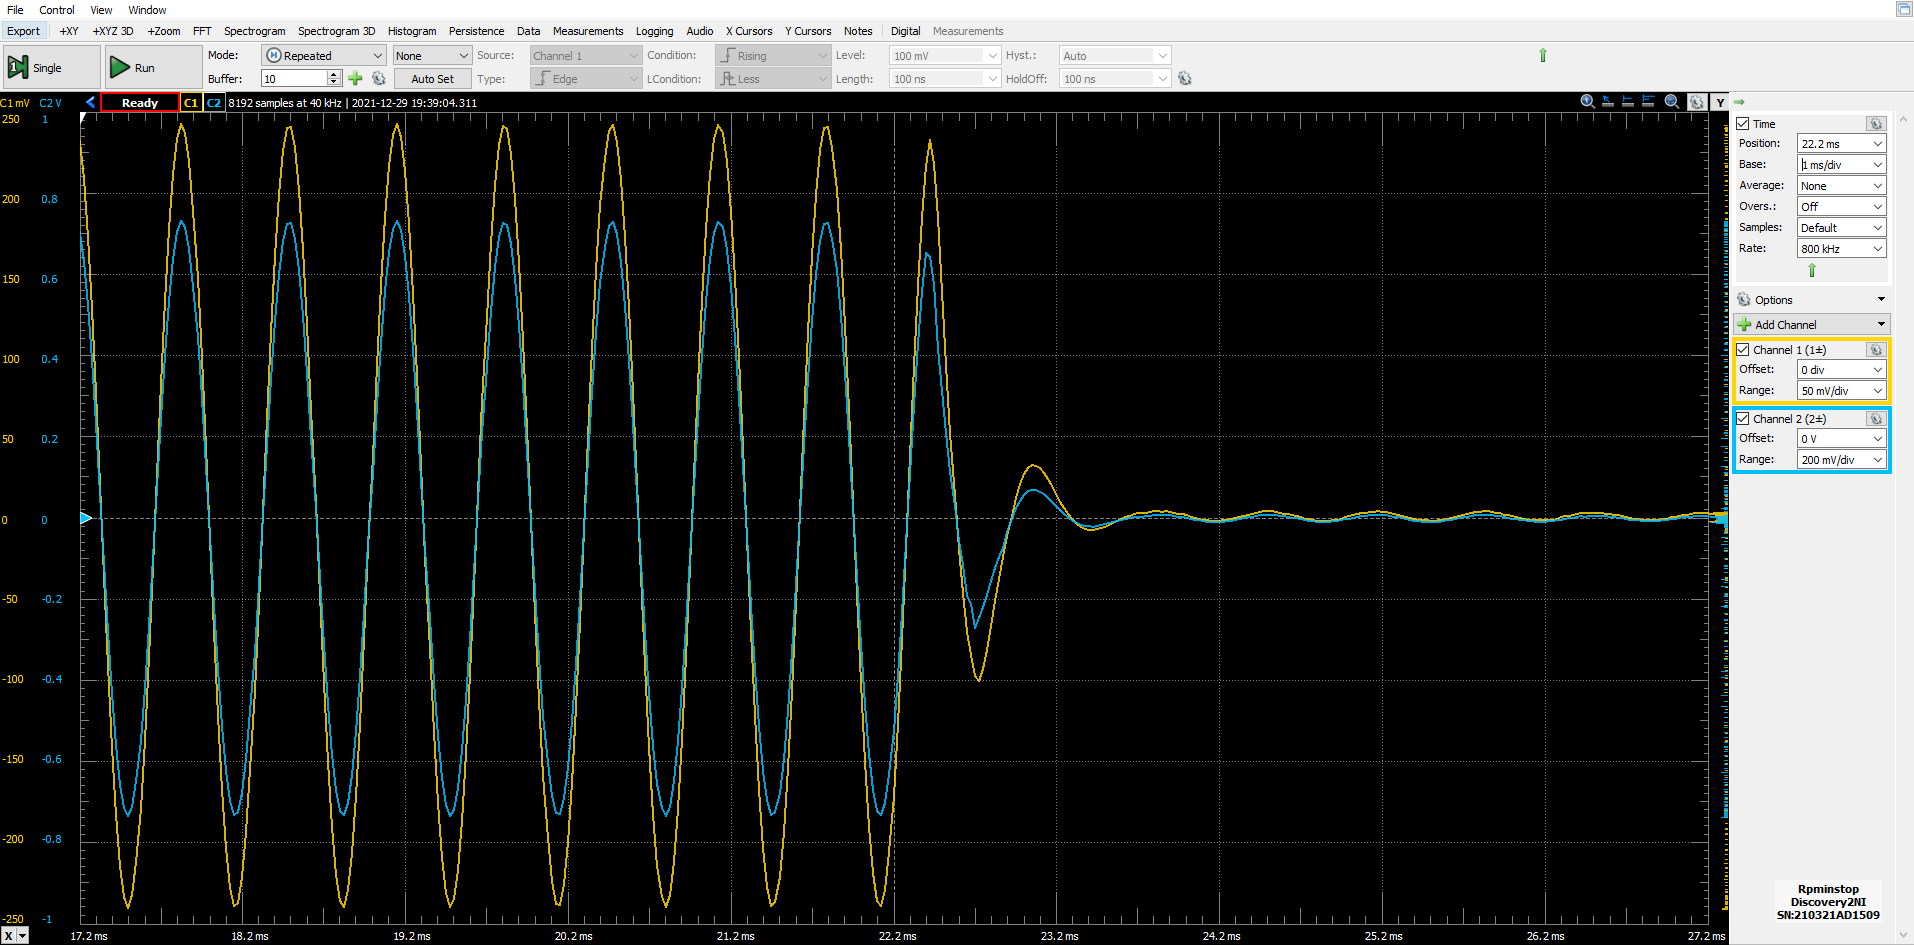
\includegraphics[width=\textwidth]{Rpminstop}
	\caption{Acquisizione dell'arresto dei segnali oscillanti $v_+ (t)$ (CH1) e
	$V\ped{out} (t)$ (CH2) non appena i diodi vengono disconnessi dal
	circuito. \label{fig: Rpminstop}}
\end{figure}

Questo perché la condizione di Barkhausen è soddisfatta solamente quando vale
$\beta A = 1$ esattamente. Ma (a causa degli inevitabili difetti fisici nei
componenti del circuito) non è possibile soddisfare questa condizione ideale
a meno che non si introduca una non linearità nella risposta -che tenda a
riportare il sistema nello stato ottimale per sostenere le oscillazioni- per
porre rimedio a questo problema facciamo uso dei due diodi.

Senza di questi, a seconda delle condizioni di lavoro del circuito, possono
succedere sostanzialmente due cose:
\begin{enumerate}
\item $|\beta A| < 1$ $\implies$ Il circuito si trova in regime stabile,
quindi non inizia mai ad oscillare. Perché se $p$ è troppo grande, cioè
tale che $A < 3 \implies L(j\omega) < 1$, dalla teoria generale sui sistemi
con feedback sappiamo che l'inviluppo di $V\ped{out}(t)$ decade
esponenzialmente nel tempo.
\item $|\beta A| > 1$ $\implies$ Il circuito è in zona instabile e
l'oscillazione diverge fino alla saturazione dell'uscita dell'OpAmp.
Perché al contrario, quando $A(p) > 3 \implies L(j\omega) > 1$,
l'inviluppo del segnale in uscita cresce esponenzialmente. In realtà la
crescita esponenziale è limitata dal \emph{voltage swing} dell'operazionale
(i.e. dal massimo valore della d.d.p erogabile, nel nostro caso come riportato
nel datasheet $\pm 13.6 \; \si{\V}$ per tensioni di alimentazione pari a
$V_{CC} = - V_{EE} = 15 \; \si{\V}$.).
\label{item: case2}
\end{enumerate}

Allora è possibile studiare l'innesco dell'auto-oscillazione grazie
all'oscilloscopio semplicemente eliminando il corto-circuito dopo aver avviato
l'acquisizione in modalità single-shot. Ne riportiamo alcuni esempi al
variare del valore della resistenza del potenziometro $Rp$, in cui come misura
della durata del transiente si è preso l'intervallo di tempo necessario perché
$V\ped{out} (t)$ cresca dal $10\%$ al $90\%$ del suo valore massimo (misurato
con i cursori dall'ampiezza dell'auto-oscillazione nel regime stabile, una
volta terminato il transiente).
\begin{figure}[htbp]
	\centering
	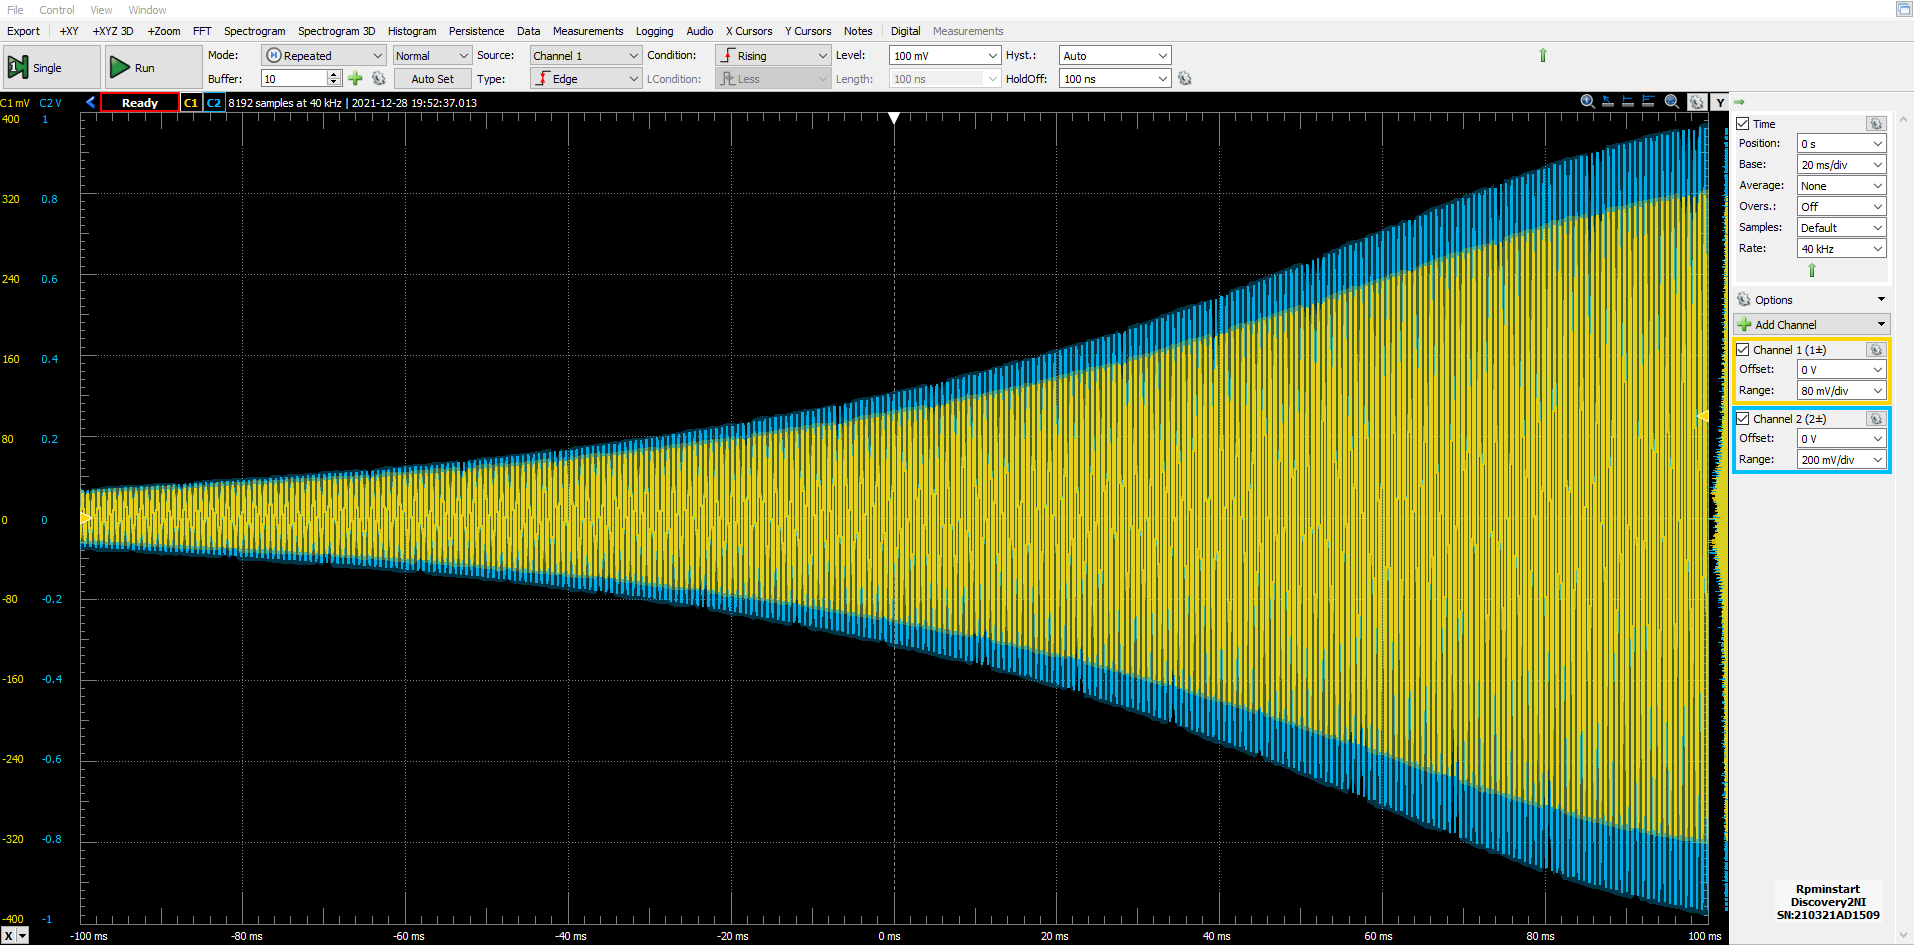
\includegraphics[width=\textwidth]{propR9}
	\caption{Acquisizione dell'innesco dell'oscillazione in $v_+ (t)$ (CH1) e
	$v\ped{out} (t)$ (CH2) quando i diodi vengono collegati nel circuito.
	Per il valore di resistenza ottimale del potenziometro
	$Rp\ped{max} = 2.96 \pm 0.03 \; \si{k\ohm}$ si registra una durata del
	transiente pari a $t = 130 \pm 2 \; \si{m\s}$.
	\label{fig: startmax}}
\end{figure}

Più è alto il guadagno dell'anello amplificatore $A(p)$ e meno tempo il
circuito impiega a raggiungere il regime di funzionamento stabile (non nullo).
Dunque ci aspettiamo che il tempo necessario perché l'oscillazione si
stabilizzi alla sua ampiezza massima sia sempre più breve al diminuire del
valore della resistenza $Rp < Rp\ped{max}$. Questo corrisponde a quanto
abbiamo osservato direttamente dalle acquisizioni in \cref{fig: start2.2V}
e \cref{fig: start3.9V}, dove il guadagno è così alto che il segnale in
uscita dall'OpAmp viene tagliato alla tensione di saturazione inferiore
$V_{OL} \approx -3.5 \; \si{\V}$.

\begin{figure}[htbp]
	\centering
	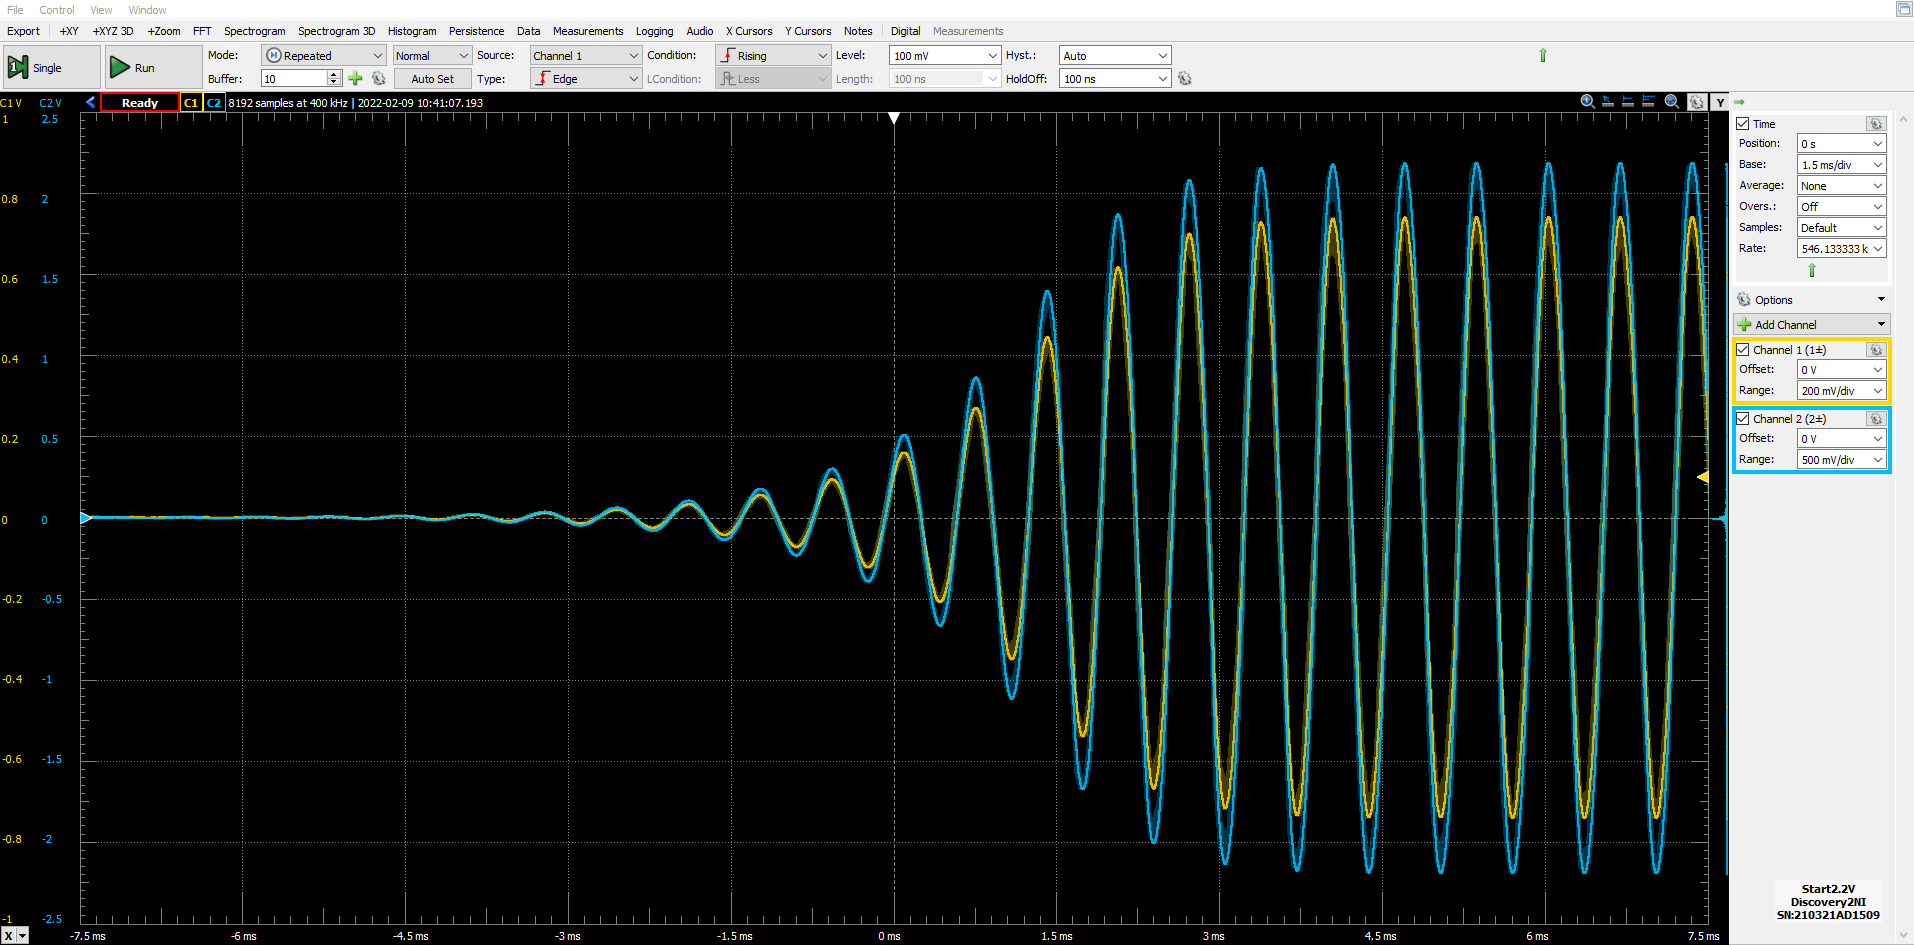
\includegraphics[width=\textwidth]{start2.2V}
	\caption{Acquisizione dell'innesco dell'oscillazione in $v_+ (t)$ (CH1) e
	$v\ped{out} (t)$ (CH2). Per un valore di resistenza del potenziometro di
	$Rp = 2.27 \pm 0.03 \; \si{k\ohm}$ si registra una durata del transiente
	pari a $t = 2.97 \pm 0.15 \; \si{m\s}$.
	\label{fig: start2.2V}}
\end{figure}

\begin{figure}[htbp]
	\centering
	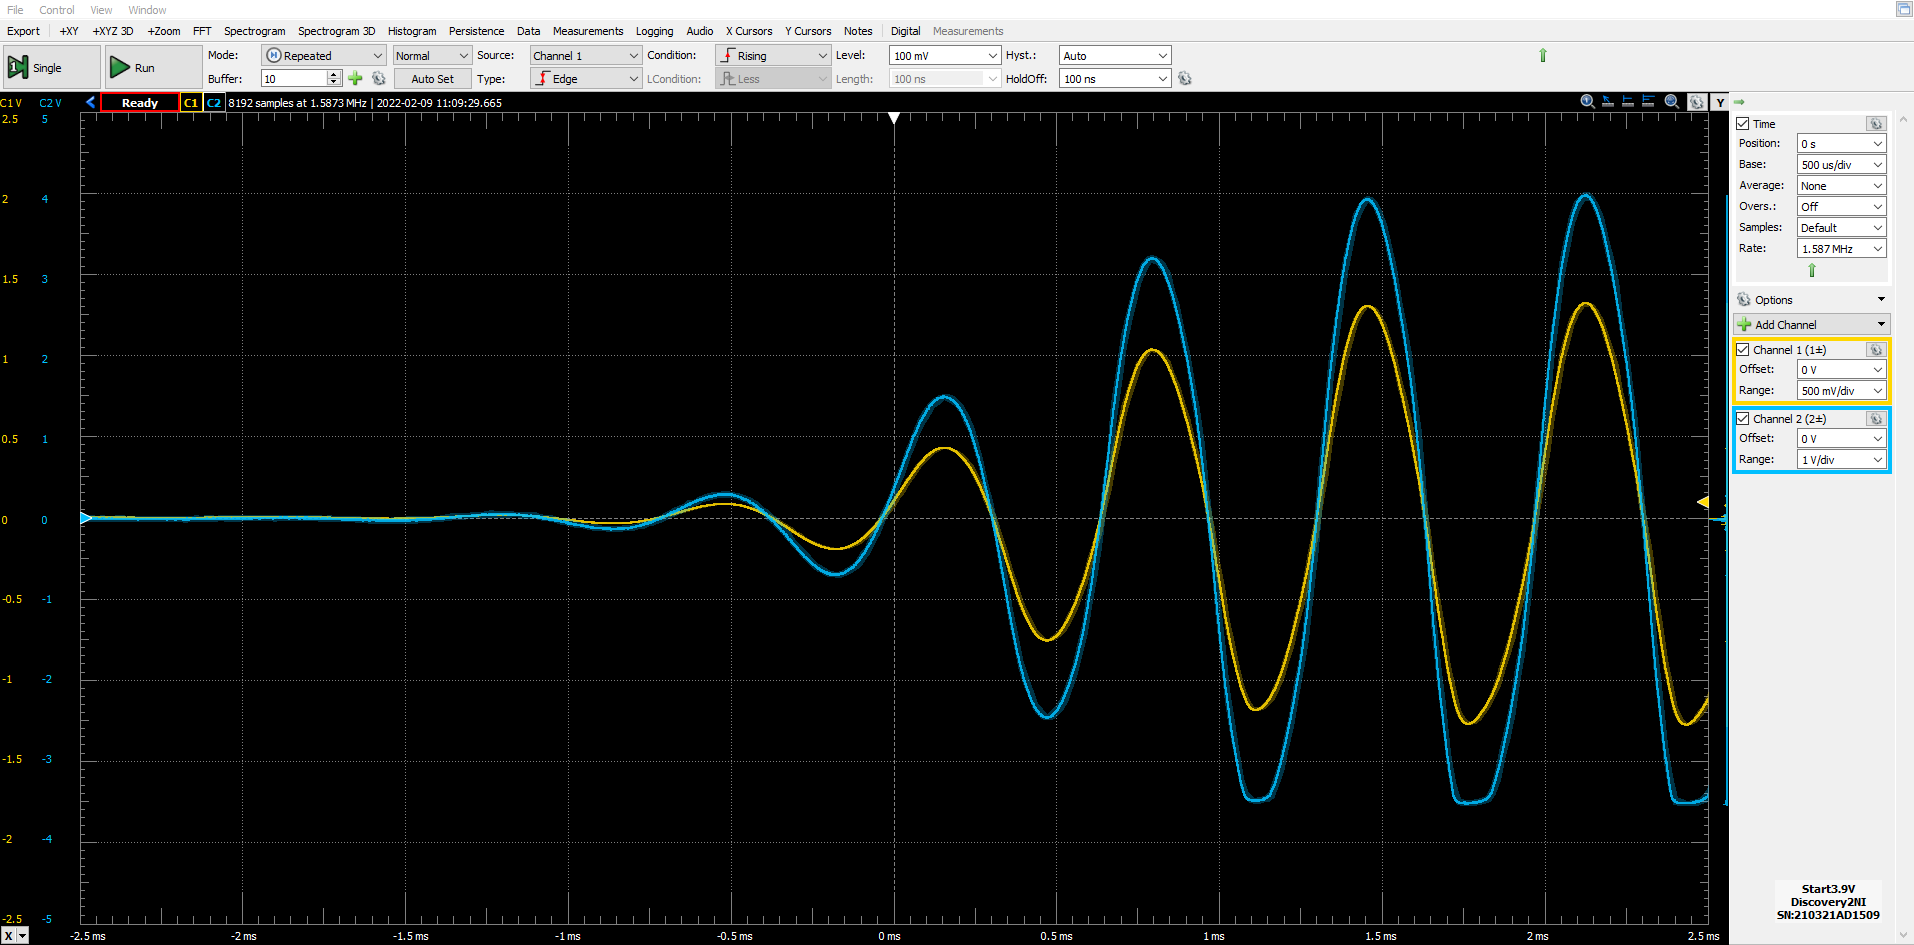
\includegraphics[width=\textwidth]{start3.96V}
	\caption{Acquisizione dell'innesco dell'oscillazione in $v_+ (t)$ (CH1) e
	$v\ped{out} (t)$ (CH2). Per un valore di resistenza del potenziometro di
	$Rp = 1.073 \pm 0.03 \; \si{k\ohm}$ si registra una durata del transiente
	pari a $t = 1.21 \pm 0.05 \; \si{m\s}$.
	\label{fig: start3.9V}}
\end{figure}

%=======================
\section{Funzione dei diodi in parallelo}
\subsection{Studio dei segnali in ingresso e uscita}
Come già accennato sopra, fintanto che la tensione ai capi dei diodi non è
abbastanza alta da farli entrare in polarizzazione diretta, nel nostro
modello il parallelo di $D1$ e $D2$ può essere assimilato ad un circuito
aperto.
Dunque per innescare l'auto-oscillazione si posiziona il contatto
strisciante del potenziometro di modo che il circuito venga a trovarsi nella
condizione descritta alla \cref{item: case2}, cioè sfruttiamo il fatto che
l'ampiezza del segnale tenderà a crescere tanto da portare i diodi in
conduzione, che a loro volta abbasseranno il guadagno fino a soddisfare la
condizione di Barkhausen.
A questo punto il segnale in uscita dall'OpAmp si stabilizza alla sua ampiezza
massima e il circuito oscilla nel regime stabile descritto nella
\cref{item: posc}.

Ripetendo il procedimento senza aver collegato i diodi invece osserviamo che
l'uscita del sistema continua a crescere in ampiezza fino a che non raggiunge
la tensione di saturazione più bassa $V_{OL}$, nonostante il parametro del
potenziometro sia come prima $p \lesssim p\ped{max} \approx 0.3$, per cui
avevamo risposta lineare in $V\ped{out} (t)$.

Questo perché la condizione di Barkhausen non è esattamente soddisfatta:
se supponiamo di avere un loop-gain leggermente maggiore dell'unità
$L(j\omega) = \beta A = 1 + \epsilon$, questo porta ad una divergenza
esponenziale del segnale in uscita, che per i limiti fisici del circuito
si traduce nella saturazione che osserviamo. Il ruolo dei diodi infatti è in
un certo senso (che discuteremo più nel dettaglio di seguito) quello di
``stabilizzare'' il segnale grazie alla resistenza dinamica del parallelo
$R_d := R_3 // D1 // D2$, dipendente dall'ampiezza di $V\ped{out} (t)$.

Questo fa sì che quando $V\ped{out}$ tende ai limiti di saturazione
$R_d \approx r_D$ (dove con $r_D \ll R_3$ indichiamo la resistenza dinamica
del diodo attivo nel semiperiodo corrispondente dell'onda in uscita)
quindi il guadagno $A$ diminuisce in modo da confinare l'OpAmp nel regime
di linearità.
Mentre nel secondo caso senza diodi $R_d \equiv R_3$, il guadagno rimane
indipendentemente dall'ampiezza $V\ped{out}$ quello atteso dall'
\cref{eq: A}, per cui il segnale può arrivare alla saturazione come osservato. 

\begin{figure}[htbp]
\centering
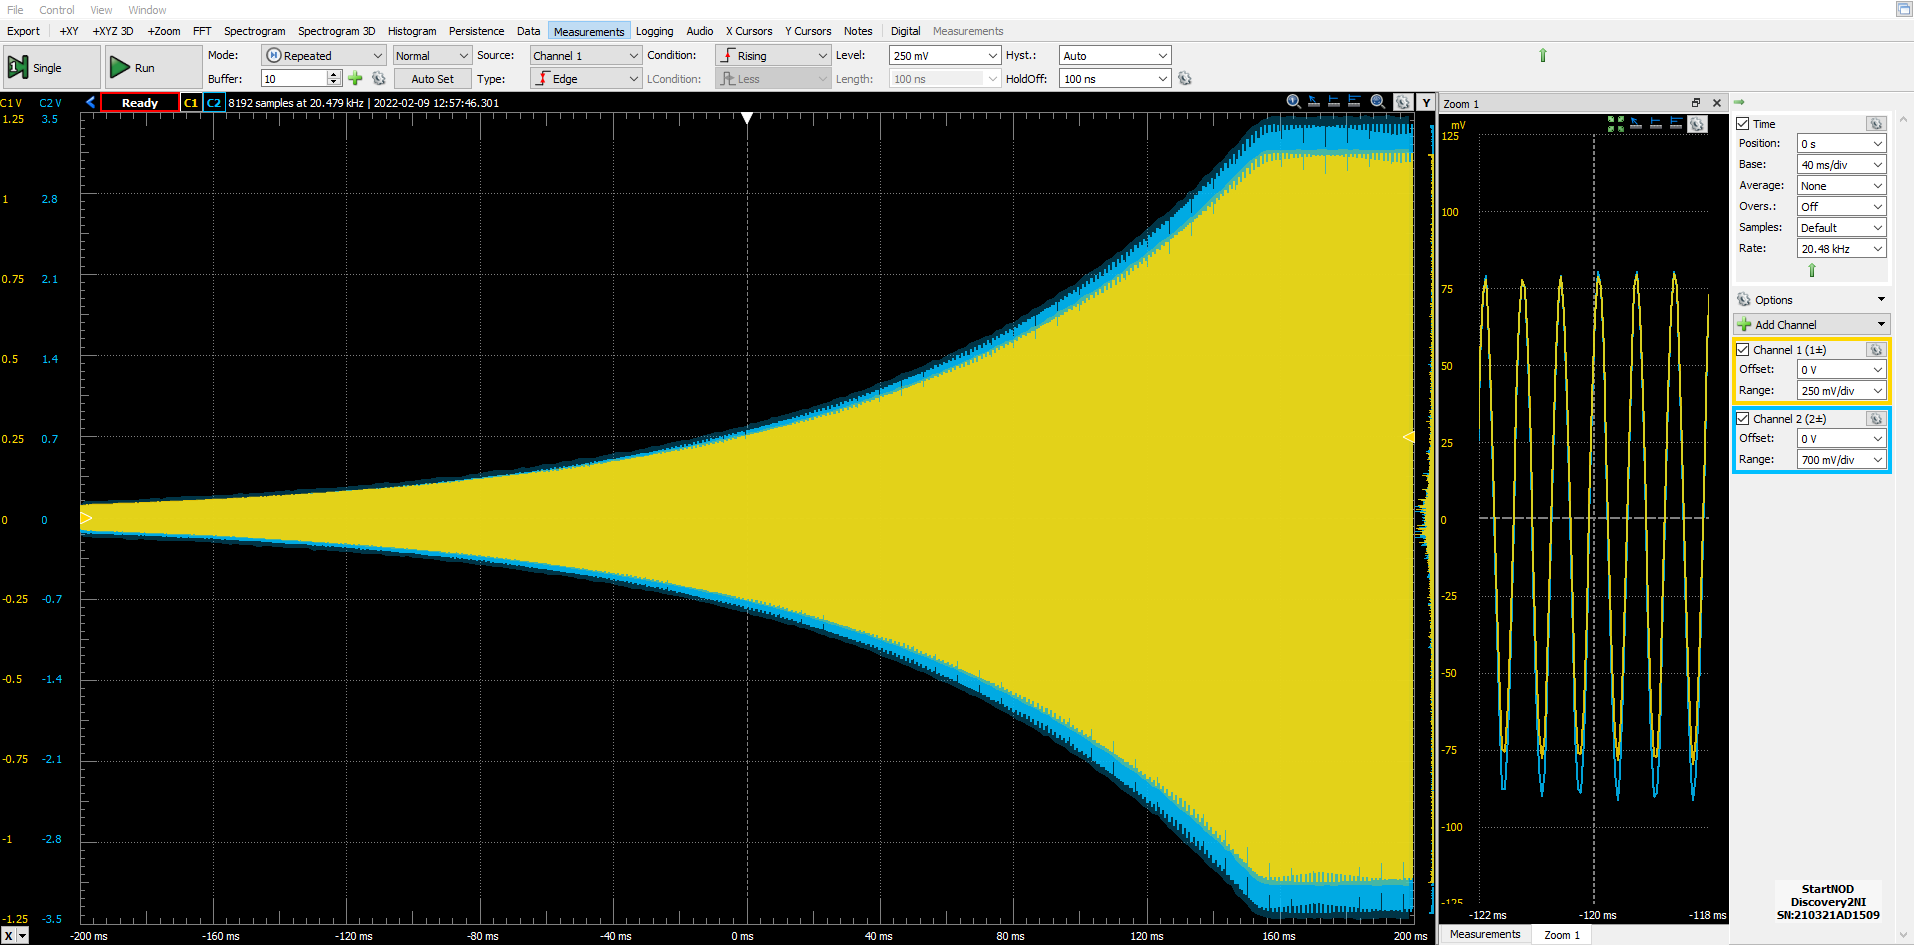
\includegraphics[width=\textwidth]{startnod}
\caption{Acquisizione dell'innesco dell'oscillazione in $v_+ (t)$ (CH1) e
	$v\ped{out} (t)$ (CH2) senza i diodi. Si nota come il segnale
	cresca esponenzialmente in ampiezza fino raggiungere il limite
	di saturazione inferiore, si può ipotizzare che questo conferisca una non
	linearità sufficiente a stabilizzare il segnale in uscita.}
\label{startnod}
\end{figure}

Si è studiata nuovamente la risposta in frequenza del circuito oscillatore in
assenza dei diodi con lo strumento Network dell'AD2 e, tramite cursore,
abbiamo rimisurato la frequenza tale per cui $\phi = 0$, che risulta identica
a quella trovata sopra. Si nota che il guadagno massimo (nello stesso punto)
è apprezzabilmente più alto di quello misurato con i diodi ($\sim - 1$ dB),
infatti ora abbiamo $A_M = |\beta(j\omega_0 \bar{A}| = 2.32 \pm 0.08 \; \si{dB}
= 1.307 \pm 0.007$

\begin{figure}[htbp]
    \centering
	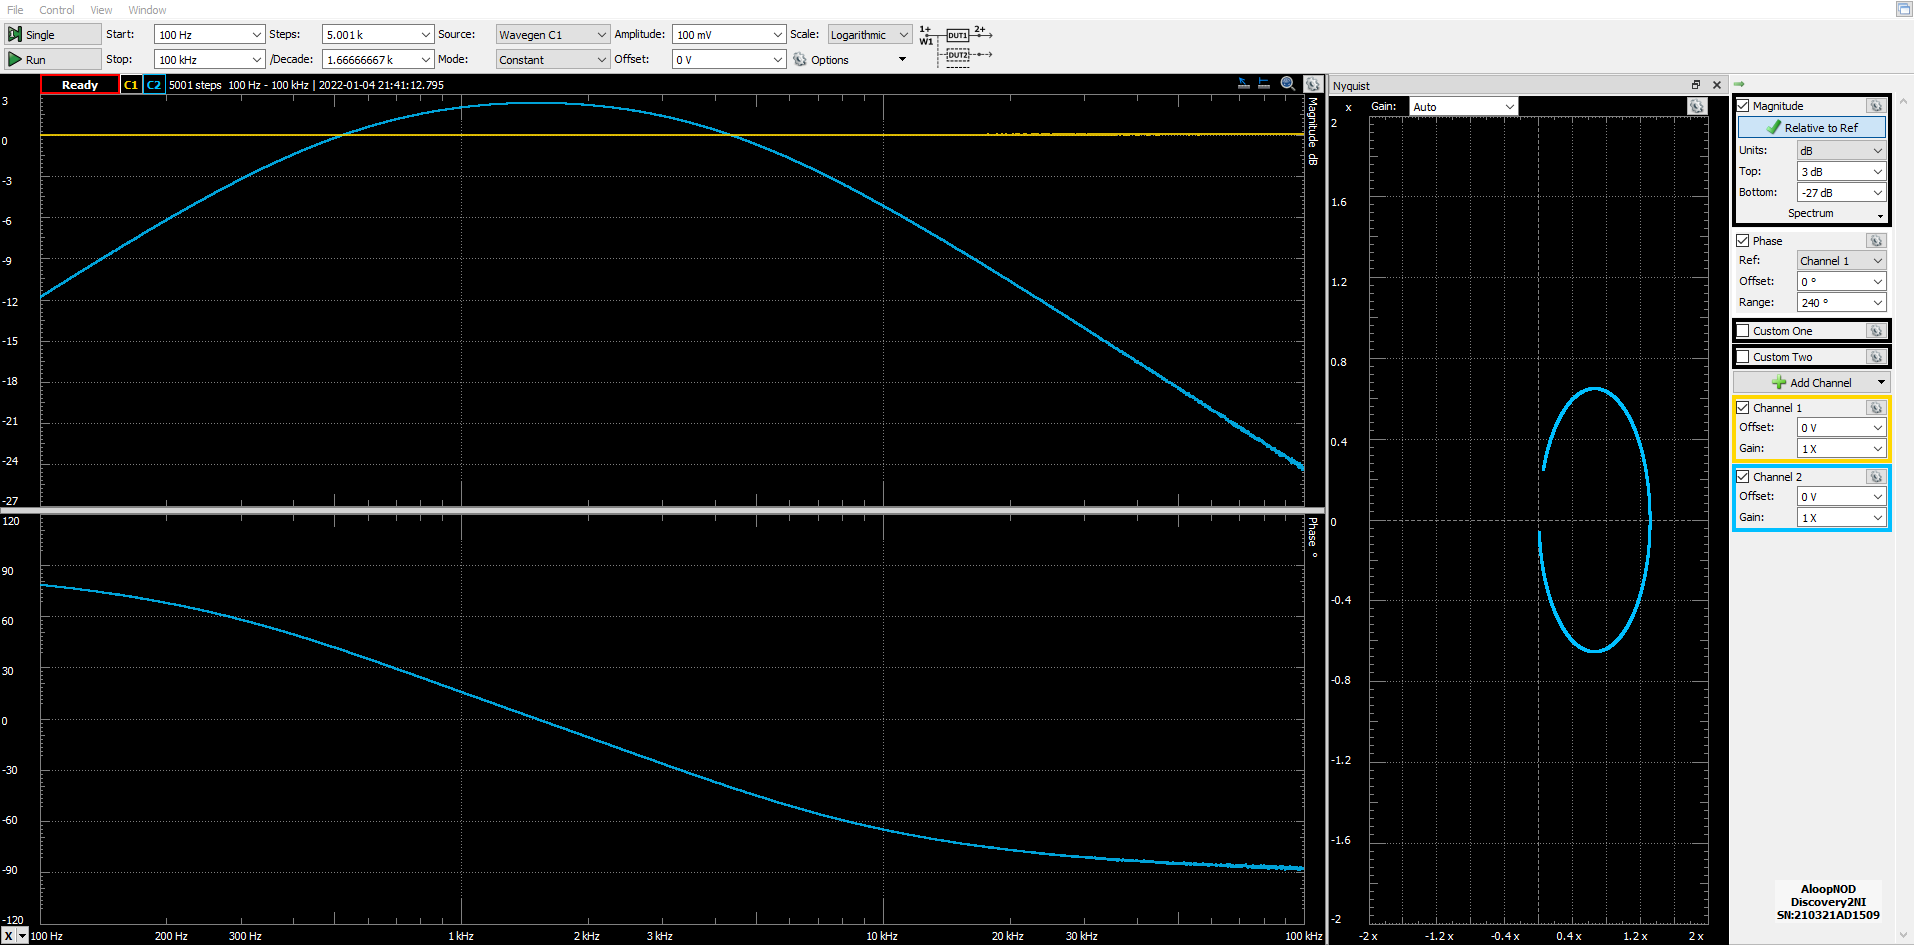
\includegraphics[width=\textwidth]{AloopNOD}
    \caption{Plot di Bode ottenuto dallo scan con Network tra
    $\SI{100}{\Hz}$ e $\SI{100}{k\Hz}$ con un segnale sinusoidale in ingresso
    all'anello di feedback invertente $A$, di ampiezza costante
    $v\ped{in} = \SI{100}{m\V}$ per il circuito senza diodi.
    \label{fig: loopnod}}
\end{figure}

\subsection{Analisi del funzionamento dei diodi}
In estrema sintesi il ruolo svolto dai due diodi è di limitare l'ampiezza
massima dell'auto-oscillazione. Poiché questa limitazione è realizzata dagli
elementi non lineari nel circuito (la coppia di diodi alternativamente in
conduzione e interdizione) ci limitiamo a dare una descrizione qualitativa del comportamento del circuito.

Come prima studiamo il caso in cui $L(j\omega) > 1$, l'inviluppo del segnale
$V\ped{out}$ cresce esponenzialmente fino a che la differenza di potenziale
ai capi dei diodi in parallelo è sufficiente a polarizzarne uno direttamente.
Supponendo di poter stimare ragionevolmente il guadagno dell'anello $A$ con la
forma del partitore
\[
A\ped{exp} = \frac{R + R_d + R_4 + R_5}{Rp + R_5}
\]
Quando i diodi entrano in conduzione, la loro resistenza abbassa il valore di
$R_d < R_3$ al numeratore, portando quindi ad una diminuzione del guadagno.
Il parallelo di diodi introduce in questa maniera un effetto di feedback
negativo che stabilizza il segnale ad una ampiezza massima (in funzione della
posizione $p$ del trimmer).

Per valori dell'ampiezza dell'oscillazione ancora più grandi di $V_\gamma$, ma
pur sempre minori del \emph{Voltage swing}, la risposta non lineare dei diodi
non è più ben descritta dal nostro modello per $A(p)$. Infatti la loro
presenza continua ad avere l'effetto di abbassare la resistenza dinamica del
ramo di feedback, ma introducono anche distorsioni nella forma d'onda in
uscita, che come abbiamo visto (anche da un'analisi in frequenza) non è più
sinusoidale.

\section{Misura di guadagno dell'oscillatore}
Come nel punto \ref{sbs: Vout/Vs} abbiamo studiato il guadagno
$A_v = V\ped{out}/V_s$ del circuito in \ref{fig: aloopschm} inviando un
segnale sinusoidale $V_s (t)$ all'ingresso positivo dell'OpAmp; una volta
fissato il terminale centrale del potenziometro nella posizione per cui si
osserva l'innesco dell'auto-oscillazione.
\begin{align*}
V_s &= 200 \pm 2 \; \si{m\V} \\
V\ped{min} &= 608 \pm 5 \; \si{m\V} \implies  A_v = 3.04 \pm 0.04
\end{align*}

Quanto trovato è compatibile con il guadagno atteso, che in queste condizioni
ci aspettiamo valga $A = 3$ per soddisfare la condizione di Barkhausen.

%=======================
\section*{Conclusioni e commenti finali}
Si è riusciti a costruire e studiare un circuito oscillatore a ponte di Wien
facendo uso di un amplificatore operazionale TL081.

In particolare siamo riusciti a descrivere e verificare sperimentalmente il
funzionamento del circuito e a caratterizzarne la risposta in uscita sia nel
dominio dei tempi che delle frequenze al variare dei parametri da cui dipende
il guadagno dell'oscillatore reazionato ad anello.

%=======================
\section*{Dichiarazione}
I firmatari di questa relazione dichiarano che il contenuto della relazione \`e
originale, con misure effettuate dai membri del gruppo, e che tutti i firmatari
hanno contribuito alla elaborazione della relazione stessa.
\end{document}
